%\newcommand\specialsectioning{\setcounter{secnumdepth}{14}} 
\specialsectioning
\chapter{物联网安全}
\label{chap:intro}

\section{引言}
\renewcommand\specialsectioning{\setcounter{secnumdepth}{2}} 
\specialsectioning
\renewcommand\sectionmark[1]{\markright{\thesection  #1}{}}

物联网的迅速崛起,带来了新一代的设备和服务。据统计,每天有超过500万个新设备连接到人们的日常生活中\footnote{Internet of Things; A Vision For The Future. https://otalliance.org/IoT}。继互联网诞生以来,这些日新月异的设备和服务,预示着一个以创新和高速增长为特征的物联网时代已经到来。物联网(Internet of Things, IoT)是一个融合计算机、通信和控制等相关技术的复杂系统,因此其面临的安全问题也更加复杂。本章主要论述物联网安全的基本概念和特征,探讨物联网安全的现状和面临的安全威胁,以及常用的攻击、防御手段。

\section{物联网安全概述}
\label{xdtz}

\subsection{什么是物联网?}
\label{IOT}

物联网其英文名称是:“Internet of things(IoT)”,从名字上看就是物物相联的互联网。关于物联网的起源,业界有不同的说法,其中一种说法是:最早的物联网设备是1991年在英国剑桥大学诞生的“特洛伊咖啡壶”。1991年,剑桥大学特洛伊计算机实验室的科学家们,经常要下楼去煮咖啡,还要时刻关注咖啡煮好了没有,既麻烦又耽误工作,于是,他们编写了一套程序,在咖啡壶旁边安装了一个便携式摄像头,利用终端计算机的图像捕捉技术,以3帧/秒的速率传递到实验室的计算机上。这样,工作人员就可以随时查看咖啡是否煮好,这就是物联网最早的雏形。

明确的物联网的概念是1999年美国麻省理工学院(MIT)的Kevin Ash-ton教授首次提出的。Kevin Ashton教授在1998年首次提出:“万物皆可通过网络相互联接”,首次阐明了物联网的基本含义,并且在麻省理工成立了“自动识别中心(Auto-ID)”,从此物联网有了基本雏形。Ashton在研究射频识别(RFID)和无线传感器网络(WSN)时提出的物联网概念,起初只是想通过RFID以及传感器技术让计算机对物理世界进行感知与识别,在无人干预的情况下汇聚数据,以此来对物品进行追踪和计数,他认为物联网与互联网一样有着改变世界的巨大潜力。


2008年,The Internet of Things in 2020报告中指出,物联网是由具有标示和虚拟个性的物体或对象所组成的网络,这些标示和个性等信息在智能空间中,使用智慧的接口与用户、社会和环境进行通信。

我国在2010年政府工作报告中,把物联网解释为:通过信息传感设备,按照约定的协议,把任何物品与互联网连接起来,进行信息交换和通信,以实现智能化识别、定位、跟踪、监控和管理的一种网络,它是在互联网基础上延伸和扩展的网络。

由此可见,物联网的概念是逐步发展和完善的,在以计算机为代表的第一次产业浪潮,以互联网、移动通信为代表的第二次产业浪潮之后,物联网正在引领信息产业的新浪潮,物联网产业蓬勃发展,极大的推动了经济发展和社会进步。


物联网技术让互联网不仅仅是延伸到最后1公里或者最后1英寸,还将无形的数字信号与有形的物理实体结合了起来。对于物联网来说,无论是作为主体还是客体,其实都可以把现实物理世界看作数字信息世界的一个直连组件。今天,物联网技术正在许多行业不断推广,并且为传统行业带来了巨大的变革。 

\textcolor{myblue}{\textbf{物联网赋能电网}}\quad 电力、天然气等公共事业公司派员工挨家挨户抄表的日子离我们越来越远了,如今的住宅都会安装一套分布式能源系统(Distributed Energy Resource, DER)系统,它可以分析电力需求和负荷数据并与配电网进行通信,进而识别出异常状态和不稳定情况,避免电压骤降和断电所付出的高昂代价。 

\textcolor{myblue}{\textbf{物联网赋能交通}}\quad
物联网已经给交通运输业带来了巨大改变,并且有望继续带来变革。\textcolor{black}{\textbf{智能交通系统}}(Intelligent Transportation System, ITS)可以发送排队预警信息,让车辆和驾驶员知道当前路段是否拥堵,然后车辆的导航系统可以针对拥堵路段迅速重新规划行驶路线,进而缓解拥堵状况。

\textcolor{myblue}{\textbf{物联网赋能智能制造}}\quad
“工业4.0”相信大家已经有所耳闻了,它主要用于描述通过自动化和数据交换来赋能智慧工厂的信息物理系统,其中涉及的用例包括远程监控、智能能耗管理、预测维护以及人机操作等,从而提高生产的灵活性。

\textcolor{myblue}{\textbf{物联网赋能智慧城市}}\quad
智慧城市是复杂物联网的一个实例,德勤最新发布的一份《超级智慧城市报告》(Super Smart City:Happier Society with Higher Quality)表示,目前全球已启动或在建的智慧城市已达1000多个,而中国在建数量大约500个,远超排名第二的欧洲(90个)。智慧城市系统通过安装若干个多功能传感器,对包括温度、气压、光线、一氧化碳、环境声强、行人和车辆的交通状况等信息进行测量,这些信息可以帮助城市管理者进行科学决策。


\subsection{物联网安全事件}
\label{computer}
任何事物都有其两面性,当我们探索物联网产业的发展机遇之时,却往往忽视了其背后的安全难题。截止到目前,因物联网设备自身漏洞被黑客攻击导致信息泄露或无法正常运行的事件依然频发,基于物联网终端的攻击事件不断见诸报端,物联网安全形势依然严峻。

2017年11月Check Point研究人员表示LG智能家居设备存在漏洞,黑客可以利用该漏洞完全控制一个用户账户,然后远程劫持LG SmartThinQ家用电器,包括冰箱,干衣机,洗碗机,微波炉以及吸尘机器人,并将它们转换为实时监控设备。2020年9月,安全公司 Avast 的研究员 Martin Hron 逆向了Smarter 公司的联网智能咖啡机,发现了很多漏洞。利用这些漏洞,他能触发咖啡机打开燃烧器、出水、启动磨豆机、显示勒索信息,并让咖啡机重复发出哔哔的声音,唯一阻止这一切混乱的方法是拔掉电源插头。Hron 发现咖啡机与智能手机应用之间的连接是没有加密的,没有身份验证,没有代码验证,最新的固件就储存在手机应用,可以很容易导出进行逆向工程。

除了家用物联网设备,车载驾驶辅助系统的安全性、可靠性也仍然未能让我们感到安心。比利时鲁汶大学(Belgian university KU Leuven)安全研究员列纳特·沃特斯(Lennert Wouters)表示,他只需大约90秒的时间,即可进入特斯拉汽车。进入车内大概1分钟左右的时间,他就可以注册自己的汽车钥匙,然后把车开走。物联网汽车不仅有被盗的风险,在驾驶中的安全性漏洞也得到了证实。《连线》杂志报道称,位于以色列内盖夫的本·古里安大学的研究人员已经证明,通过被劫持的互联网广告牌,就可诱导特斯拉电动汽车的 Autopilot 等系统采取突然的制动、驻车或转弯等操作。具体说来是,这些图像可能让自动驾驶/ 驾驶辅助系统紊乱,通过营造瞬间的光线投射,让系统“看到”不存在的物体(比如停车指示牌),从而让车辆系统做出反应。如果在恰当的时机实施这种攻击,会对车辆以及驾乘人员的安全造成严重威胁。

从提出“智慧城市”概念至今,在短短的10年内,智慧城市已经遍地开花。近日,IBM发布了一份网络安全白皮书,公布了其X-Force Red团队与安全业者Threatcare对智能城市所使用的主要系统的调查结果:共发现了17个安全漏洞,更严重的是,黑客可以通过这些漏洞任意摆布水位传感器,以触发错误的洪水警报,或是避免触发洪水警报,同样地,黑客也能操纵核电厂附近的辐射传感器,或者是借助对交通系统、建筑物警报系统或紧急警报系统的控制来制造混乱,这很可能对缺乏安全防范体系的智慧城市造成严重伤害。

以上的案例共同反映出了一个问题,那就是虽然物联网将许多的“不可能”变为了“可能”,但是在物联网产业建设初期,安全,作为物联网应用最基础保障,其防护体系的建设仍然任重道远。


\subsection{物联网安全特点}
\label{computer}

与传统意义上的网络安全不同,物联网安全是网络安全与其他工程学科相融合的产物。相比于单纯的数据、服务器、网络基础架构和信息安全,物联网安全的内涵要更加丰富。通常情况下,“网络安全”并不关注硬件设备以及同硬件设备交互的现实物理世界的物理安全和信息安全隐患,而正是通过网络对物理世界处理流程的数字化控制,使得物联网安全与传统安全有所区别,即物联网安全不再仅仅局限于包括机密性、完整性、不可否认性等基本信息安全保证原则,还需要对现实世界中收发信息的实体资源和设备进行安全保障。

物联网的安全特点主要体现在以下3个方面:

(1)安全体系结构复杂

物联网海量的感知终端,使其面临复杂的信任接入问题;物联网传输介质和方法的多样性,使其通信安全问题更加复杂;物联网感知的海量数据需要储存和保存,这使得数据安全变得十分重要。因此,构建合适全面、可靠传输和智能处理的物联网安全安全体系是物联网发展的一项重要工作。

(2)安全领域覆盖广泛

物联网所对应的传感器网络的数量以及其连接的智能终端规模巨大,这种体量是单个物联网传感器是无法比拟的,这会引入更复杂的访问控制问题;其次,物联网所连接的终端设备或器件的处理能力有很大差异,他们之间会相互作用,信任关系复杂,需要考虑差异化系统的安全问题;最后,物联网所处理的数据量将比现在的互联网大很多,需要考虑复杂的数据安全问题。

(3)有别于传统的信息安全

与传统意义上的网络安全不同,物联网安全是网络安全与其他工程学科相互融合的产物,相比与单纯的数据、服务器、网络基础架构的信息安全,物联网安全的内涵要更加丰富。在物联网环境中,即使分别确保了物联网各个层次的安全,也不能保证物联网整体的安全,这是因为物联网是融合多个层次于一体的大系统,许多安全问题来源于系统整合。例如,物联网的数据共享对安全性提出了更高的要求,物联网的应用需求对安全提出了新的挑战,物联网的用户终端对隐私保护的要求也日益复杂。

鉴于以上的安全特点,物联网的安全体系需要在现有信息安全体系之上,制定可持续发展的安全架构,使物联网在发展和应用过程中,其安全防护措施能够不断完善。

\subsection{物联网安全体系结构}
\label{computer}

在物联网系统中,主要的安全威胁来自以下几个方面:物联网传感器节点接入过程中的安全威胁、数据传输过程中的安全威胁、物联网数据处理过程中的安全威胁、物联网应用过程中的安全威胁等。这些威胁时全方位的,不管安全威胁的来源是哪些,我们都可以将物联网的安全需求归结为以下几个方面:物联网感知安全、物联网接入安全、物联网通信安全、物联网数据安全、物联网隐私安全。根据以上的需求,我们可以构建一个以需求驱动的物联网安全体系,具体包括以下内容:
\subsubsection{\textcolor{myblue}{\textbf{1. 物联网感知安全 }}}

物联网感知层的核心技术涉及传感器、条形码和RFID等技术,传感器在输出电信号时,容易受到外界干扰甚至破坏,从而导致感知数据错误、物联网系统工作异常等问题。例如,RFID技术使用电磁波进行通信,并且储存着大量数据,攻击者有可能通过窃听电磁波信号“偷听”传输内容,进而达到各种非法目的。

显然,物联网的感知节点接入和用户接入离不开身份认证、访问控制、数据加密和安全协议等信息安全技术。

\subsubsection{\textcolor{myblue}{\textbf{2. 物联网接入安全 }}}

在接入安全中,感知层的接入安全是重点。一个感知节点不能被未经认证授权的节点或系统访问,这涉及到节点的信任管理、身份认证、访问控制等方面的安全需求。另外,由于传感器节点受到功率和功能的制约,其安全保护机制交叉,其中的消息和数据传输协议没有统一的标准,从而无法提供一个统一、完善的安全保护体系。因此,传感器网络除了可能遭受与现有互联网相同的安全威胁外,还可能会受到恶意节点的攻击、传输的数据被监听或破坏、数据的一致性差等安全威胁。

另外,物联网授权要求信息在接入和传输过程中保证完整性,未经授权不能改变。即信息在存储或传输的过程中不被偶然或蓄意删除、篡改、伪造、乱序、重放等操作造成破坏和丢失。这时候还需要利用数字签名、加密传输等技术手段保持信息的正确生成、存储和传输。

\subsubsection{\textcolor{myblue}{\textbf{3. 物联网通信安全 }}}

物联网依靠通信终端来获取数据,目前的智能终端数量呈指数增长,而现有的通信网络承载能力有限,当大量的网络终端节点接入现有网络时,将会给通信网络带来更多的安全威胁。首先,大量终端节点的接入肯定会造成网络拥塞问题,给攻击者可乘之机。其次,由于物联网中设备传输的数量较小,为了降低功耗提高效率,很多通信协议都是明文传输(MQTT协议等),可能导致数据在传输过程中遭到攻击和破坏。

\subsubsection{\textcolor{myblue}{\textbf{4. 物联网数据安全 }}}

随着物联网的发展和普及,物联网数据呈爆炸式增长,在这种情况下,云计算、大数据等技术应运而生。虽然这些新型计算模式解决了个人和组织的数据处理需求问题,但同时,也增加了数据失控的危险。因此,针对数据处理中的安全隐私保护技术显得尤为重要。物联网安全审计要求物联网具有保密性和完整性,保密性要求信息不能泄露给未授权的用户,完整性要求信息不受各种破坏。

\subsubsection{\textcolor{myblue}{\textbf{5. 物联网隐私安全 }}}

除了上述安全指标之外,物联网中还需要考虑隐私安全问题。当今社会,无论是公众人物还是普通人,保护个人隐私已经成为了广泛共识。根据国家保密局发布的信息显示,物联网直接暴露于互联网,很容易遭受网络攻击,近20\%的企业或机构在过去的3年内遭受了至少一次物联网攻击,用户隐私也因此遭受着较大的泄露风险。在物联网隐私问题中,包含用户的信息隐私和位置隐私两个方面,信息隐私问题主要是指物联网中数据采集、传输和处理等过程中的秘密信息泄露,它往往与数据安全密不可分,因此一些信息隐私威胁可以通过数据安全的方法解决。位置隐私是物联网隐私保护的重要内容,主要指物联网中各节点的位置隐私以及物联网在提供各种位置服务时面临的位置泄露问题,具体包括RFID阅读器位置隐私、RFID用户位置隐私、传感器节点位置隐私以及基于位置服务中的位置隐私问题。


\subsection{物联网安全挑战}
\label{computer}

与传统网络相比,物联网发展带来的信息安全、网络安全、数据安全乃至国家安全问题将更加突出,我们要强化安全意识,把安全放在首位,超前研究物联网产业发展可能带来的安全问题。物联网除了要解决传统的安全问题之外,还需要克服认证接入、隐私保护等新的挑战,具体介绍如下:

\subsubsection{\textcolor{myblue}{\textbf{1.针对物联网的攻击增加}}}

卡巴斯基安全专家 Dan Demeter 表示:“由于物联网设备的发展,从智能手表到智能生活配件,已经成为我们日常生活中必不可少的一部分,网络犯罪分子巧妙地将注意力转移到了这一领域。” 由于物联网连接更多的智能终端,也会获取更多的隐私数据,相比互联网来说更加深入我们的生活,所以物联网与互联网的攻击方式有所区别。

本章\textcolor{myblue}{\textbf{第二节:针对物联网的特定攻击}}将结合物联网的特点,从物理设备层面和系统固件层面详细介绍针对物联网的攻击种类、效果以及造成的危害,最后介绍了针对一些特定攻击的前沿研究成果。

\subsubsection{\textcolor{myblue}{\textbf{2. 物联网协议安全性低}}}

目前物联网通信协议仍然存在许多严重的安全问题\cite{ref1},有些研究\cite{ref2,ref3,ref4}表明了物联网协议栈中链路层存在安全漏洞,攻击者可以发起时间同步攻击、篡改攻击和能量耗尽攻击等。也有研究者\cite{ref5,ref6}指出了物联网协议栈中 RPL协议存在多种 安全漏洞,攻击者可以发起女巫攻击、选择前向攻击、HELLO 洪泛攻击以及虫洞攻击等,从而破坏 RPL协议正常运行。

本章\textcolor{myblue}{\textbf{第三节:物联网网络协议安全}}将介绍现有的物联网通信协议,分析现有协议的用途以及其安全缺陷,介绍目前的前沿研究方向。

\subsubsection{\textcolor{myblue}{\textbf{3.物联网设备的认证与授权机制不完善}}}

Zscaler公司最近发布了其第二份年度物联网报告,报告中对212个制造商的21种不同的共计553种IoT设备进行了统计分析。其中最让人担忧的是“影子物联网”的存在,世界各地的企业、机构都在观察这种影子物联网现象,即员工将未经授权的设备带入企业,连接网络进行办公,这些未知和未经授权的设备给网络系统带来了巨大的安全隐患。报告中还指出,未经授权的物联网设备数量上升趋势明显,针对未经授权设备的新攻击不断涌现。

本章\textcolor{myblue}{\textbf{第四节:物联网设备的认证与授权}}将介绍现有的物联网设备的认证与授权方案,围绕非法接入和非法访问分析现有方案的安全缺陷,然后介绍目前的研究方向以及研究成果。

\subsubsection{\textcolor{myblue}{\textbf{4.物联网隐私泄露问题堪忧}}}

近年来,随着GDPR(General Data Protection Regulation)等法律法规框架日益受到重视,以及网络威胁形势变得更加动态和复杂,如何更好地保护敏感数据和个人数据隐私的问题变得日益突出。物联网(IoT)正在改变多个行业,但同时,物联网需要使用智能终端等设备收集大量的数据并对其进行分析,所以不可避免的在数据隐私方面带来了一些挑战。

本章\textcolor{myblue}{\textbf{第五节:物联网隐私保护}}将介绍目前物联网隐私保护面临的新情况与新挑战,然后介绍物联网隐私数据的具体分类,最后介绍现有的物联网轻量级隐私保护技术与目前物联网隐私保护领域的最新成果。


\section{针对物联网的特定攻击}
\label{specific-attack}

物联网技术不断发展变革,深刻影响着传统产业形态和人们的生活方式。通过泛在对象设备化、自治终端互联化、普适服务智能化,物联网收集、存储、分析海量数据用于提供即时、便捷、普适的智能化服务,在智慧城市、智慧金融、智慧医疗、智慧农业、智慧交通等诸多领域展现出了无与伦比的发展前景。然而,随着数以亿计的设备接入物联网,加之终端设备自身异质性、分散性、脆弱性的特点,整个生态体系中针对物联网的特定攻击和欺骗行为大量涌现,严重威胁着物联网安全。一是在\textcolor{myblue}{\textbf{物理设备层面}},物联网具有开放包容的特性,各种异构终端自主互通互联、共享数据,丰富的设备类型和庞大的网络流量为侧信道攻击提供了可行条件,攻击者可通过各种隐匿的侧信道轻易窃听、篡改、伪造数据从而造成数据泄露和污染;二是在\textcolor{myblue}{\textbf{系统固件层面}},泛在部署的物联网设备受限于计算、存储和网络资源,针对系统固件缺乏强有力的安全保护机制和自适应的漏洞检测手段,因而设备本身的固件漏洞仍然是其遭受威胁的主要因素。本节将从物理层侧信道威胁和系统级固件脆弱性两方面切入,综合介绍针对物联网的特定攻击及其前沿研究。


\subsection{物理层侧信道威胁}
\label{side-channel}

物联网设备使用过程中,会接收或者发送各种模态的信号。例如,在智能音箱在接收端,需要分析语音信号中的控制指令;在发送端,需要播放声音信号。而麦克风与扬声器作为发送端与接收端的两种重要传感器,除了能够处理声音信号之外,还会泄露振动信号、电磁信号等其他模态的信号。

正是因为物联网设备会接收或者泄露多种模态的信号,出现了五花八门的侧信道攻击,这些攻击针对的不是物联网设备使用的主要信道,而是伴随主要信道产生的次要信道,从而实现信息注入或者读取的目的。例如,对于重要的输入设备“键盘”,出现了利用键盘敲击声音的推测出键盘敲击内容的侧信道攻击;对于智能语音助手的接收设备麦克风,出现了利用超声波注入语音指令的侧信道攻击;对于涉及WiFi信道的路由器,出现了利用WiFi信道窃听人体语音的侧信道攻击。

这些侧信道攻击往往难以预防,这是由于这些被攻击的物联网设备在制造之初,没有考虑侧信道攻击的威胁。对于键盘,从声音信道泄露的键盘敲击声不会被刻意消除;对于智能语音助手的麦克风,从超声波信道注入的语音命令难以被滤除;对于本来用于传递数据信息路由器,从WiFi信道中感知人体语音信息的行为难以被阻止。


\subsubsection{\textcolor{myblue}{\textbf{1. 基于机械波的攻击 }}}

在物联网系统中,智能语音设备处于控制中心的地位,用户通过智能语音助手,可以控制其他设备。因此一旦智能语音设备被攻击,物联网系统的安全就会受到威胁。麦克风与扬声器作为智能语音设备中的重要输入输出传感器,接收与处理的信号主要是机械波。在无法察觉的情况下,机械波中容易嵌入恶意信息,从而威胁智能语音系统的安全。

基于机械波的攻击有多种手段。第一种是超声波攻击,攻击者将正常频率范围的语音信号调制成人体无法听到的超声波信号,然后使用超声波发射器发射调制后的超声波信号,从而实现对智能语音设备的攻击。这种攻击利用了麦克风设备本身的非线性,将隐藏在超声波信道中的语音命令恶意注入麦克风,由于麦克风会将这种超声波识别成正常语音,智能语音设备会被恶意控制。第二种是振动攻击,攻击者将承载智能语音设备的固体作为媒介,通过固体振动的频率来传输语音命令,从而实现对智能语音设备的控制。

\subsubsection{\textcolor{myblue}{\textbf{2. 基于电磁波的攻击 }}}
除了使用机械波进行交互的设备之外,还有一部分设备使用电磁波进行通信。无线路由器可以使用Wi-Fi信号实现信息的交换,毫米波雷达可以使用毫米波信号实现距离的测量与定位。这类主动式传感设备在使用电磁波的信号完成本职工作的同时,信号中还会嵌入所处环境下的额外信息。

攻击者有多种基于电磁波的攻击手段。首先是Wi-Fi攻击,攻击者使用Wi-Fi信号感知人体口腔运动的细粒度变化,并通过机器学习的方法从中分析出语音的内容,从而实现对人体的窃听。然后是毫米波攻击,攻击者使用毫米波信号感知液晶显示器的状态变化,建立模型分析电子屏幕的内容,从而实现对电子屏幕的监测。

\subsection{系统级固件脆弱性}
\label{firmware}
系统级固件的脆弱性,普遍存在于各种计算设备上,包括超级计算机,个人计算机,以及各种物联网设备。从人们意识到固件的脆弱性开始,不断有一些防御的方案被提出,个人计算机和超级计算机越来越被难以攻破,但是对于物联网设备而言,由于种种局限性,目前系统级的固件脆弱性仍是较大的安全威胁。

物联网设备的固件局限性体现在多方面,第一,由于对固件调试以及检测的有效工具较为缺乏,所以有大量携带漏洞的固件存在于实际产品;第二,由于计算能力,内存资源等限制,许多防御的机制例如数据执行保护,地址随机化等无法部署,缺乏安全保护机制的情况下,漏洞可以轻易地被攻击;第三,由于物联网设备固件大多是由第三方设计开发,不会考虑对固件代码的更新,所以即使有漏洞被发现,大量已经部署的设备并不能自动更新代码以修复漏洞。

总的来说,由于缺乏固件调试工具,所以实际产品中存在大量携带漏洞的固件,并且由于第三方不提供更新固件代码服务,即使漏洞被发现,实际产品的固件也不能被修复,最后由于物联网设备本身计算能力和内存资源的局限性,无法部署安全保护机制,导致漏洞可以被轻易利用,进而导致设备本身被成功攻击,引发一系列安全问题。下面我们介绍一些常见的固件相关的漏洞和威胁。


\subsubsection{\textcolor{myblue}{\textbf{1. 内存漏洞 }}}
固件内存漏洞一般由编写代码时的错误引起,会导致对内存的非法访问、控制流劫持等攻击。由于物联网设备固件主要由较为底层语言(例如C语言)编写,在开发过程中会不可避免地引入编码缺陷。硬件层面,物联网设备具有异构性,多样性等特点,使得对固件程序开展规模化和自动化的漏洞检测十分困难;软件层面,由于有限的硬件资源,导致必要的防御机制无法被部署,攻击者更加容易利用内存漏洞\cite{SecSurvey}。

当内存漏洞被发现时,攻击者有多种利用手段。第一种是代码注入\cite{InjectRobot},攻击者可以利用内存漏洞,将一些关键代码注入到内存数据区,进而使漏洞程序运行攻击者设计的代码,通常在个人计算机上,有数据不可执行等防御措施,可以很好地对代码注入进行防护;第二种是控制流劫持\cite{muRAI},攻击者通过利用内存漏洞,可以修改函数返回地址,并且在堆栈上任意构造函数输入,进而劫持目标程序的控制流,通常在个人计算机上,有地址随机化,控制流完整性保护等防御措施,可以对控制流劫持进行保护。此外,攻击者也可以结合其他攻击手段,比如通过对固件二进制进行逆向工程,得到一些关键的敏感控制数据,然后结合得到的控制数据和内存漏洞,对程序权限进行修改,达到攻击目的。

\subsubsection{\textcolor{myblue}{\textbf{2. 逻辑漏洞 }}}
固件逻辑漏洞也是一种常见的固件漏洞,指的是固件在认证、授权、应用功能等方面的设计或实现缺陷。通常,攻击者会利用逆向工程的手段,从固件二进制代码中寻找逻辑漏洞,当攻击者找到代码的逻辑缺陷后,只需要构造特定的输入,就可以使得程序在正常运行的同时,功能发生偏移。比如认证绕过漏洞\cite{PriviSep},就是一个典型的固件逻辑漏洞类型,攻击者通过这种漏洞来绕过系统对于特权指令的权限检查,来实施非法恶意的行为;在智能网络打印机固件程序中的逻辑设计缺陷,在实际的办公场景中会造成任务篡改、机密泄露等后果\cite{ExpPrinter}。


\subsection{前沿研究}

\subsubsection{\textcolor{myblue}{\textbf{1. 侧信道威胁 }}}
无线电通信技术广泛应用在物联网系统当中,而无线电除了能够传输数据信息,在传输过程中还会与物体产生反射,从而携带了部分额外的信息。Wi-Fi信道作为在我们日常生活中不可或缺的信道,其安全性值得被探索与研究。目前许多的工作使用Wi-Fi信号实现了对人体的窃听、运动监测、手势识别、与定位。WiTrack\cite{witrack}利用从用户身上反射的WiFi信号,追踪用户在三维空间中的运动,并提供对人身体各个部位的粗略追踪。WiHear\cite{wihear}依据人体在说话过程中,Wi-Fi信号能够感知到口腔特定的运动轮廓的特点,使用信号处理技术捕捉Wi-Fi信号中人体嘴部产生的微小反射,并利用机器学习的手段,将Wi-Fi信号中的隐藏的口腔运动特征识别成对应的音节,从而实现对人体的窃听。这类基于Wi-Fi信号的侧信道攻击,不容易受到障碍物的影响,而且由于目前Wi-Fi信号广泛被部署,往往无需额外配置设备,难以防范。

激光作为另一种重要的电磁波,在通信、工业、军事等领域发挥了巨大的作用,而目前出现了许多利用激光信号实现的侧信道攻击工作。LightCommands\cite{lightcommands}依据麦克风会对光信号做出反映的特点,通过调节激光的振幅,远距离向麦克风注入激光信号来模拟声音,从而影响智能语音设备,实现对语音系统的控制。Rolling Colors\cite{rolling colors}针对CMOS相机设备的固有弱点,在相机捕捉的图像中注入特殊的图像模式,从而干扰交通灯识别系统的准确性,威胁自动驾驶车辆的行驶安全。


\subsubsection{\textcolor{myblue}{\textbf{2. 固件脆弱性 }}}

物联网设备多种多样,其中工业机器人是一类比较典型的设备。工业机器人在工业上有着大量的应用,并且有着很高的市场市值,一般地,它是由软件控制,与物理世界进行交互的。相关研究\cite{InjectRobot}表明,由于计算机连通性的不断增强,本应该在网络独立环境下工作的工业机器人,基本上被暴露在外界网络,但是在工业机器人重要性与日俱增的同时,其背后的软件实现却增加了安全性的隐患。在现实工业环境中,当前许多种工业机器人会通过FTP服务器暴露在互联网。此时,通过互联网远程对工业机器人背后的控制软件进行侵入,进而影响工业机器人与物理世界的交互行为,最终可以实现攻击操作员或是工业机器人附近人类。也就是说,通过攻击本身具有与物理世界交互能力的物联网设备其背后的软件漏洞,可以造成对物理世界的真实威胁。

其他最新的研究更多地集中在防御上,人们试图通过编译器来保护物联网设备上的裸机程序,或其他手段来帮助检测固件漏洞。裸机的物联网设备,由于没有操作系统来管理权限和硬件资源,这导致攻击者一旦攻破程序本身,就可以直接拥有对各种硬件资源的访问权限,这是裸机程序缺乏权限管理的直接后果。一方面,人们试图提出一种新的基于LLVM的编译器\cite{PriviSep},在编译时识别需要权限的指令,并加以保护。另一方面,人们希望通过在基于微控制器的物联网设备固件上增加返回地址的完整性保护\cite{muRAI},以防御传统的控制流劫持攻击。












\section{物联网网络协议安全}
\label{protocol_security}

\par 在物联网系统中,通信设备依靠网络协议来提供服务,确保这些协议的安全性与可靠性势在必行。事实上,物联网协议安全对于物联网的存在与事物本身一样重要。但是,由于不同环境的功能差异以及标准操作系统的缺失,物联网生态系统面临着多种数据内容与形式,这一多样性使得开发适用于各种物联网设备和系统的标准安全协议变得困难。
\par 依照适用范围来看,物联网领域的通信协议主要分为以Bluetooth为代表的\textcolor{myblue}{\textbf{物联网通用网络协议}}和以NB-IoT为代表的\textcolor{myblue}{\textbf{物联网专用网络协议}}。本节主要介绍常见的物联网通信协议与安全机制,以及相关领域的前沿工作进展。

\subsection{物联网通用网络协议安全}
\label{common_security}

\subsubsection{\textcolor{myblue}{\textbf{1. Bluetooth}}}
\par 蓝牙(Bluetooth)是一种短距离无线通信标准,主要工作在2.4GHz的\textcolor{myblue}{\textbf{ISM频段}}\snote{该频段主要向工业,科学和医学领域开放,无需授权,免费使用},采用分散式网络结构以及快调频和短包技术,能够实现全双工通信。由于具有低功耗、低成本、抗干扰等特点,蓝牙耳机、蓝牙手环、车载蓝牙等设备无一不在影响人们的日常生活,蓝牙技术已广泛应用于语音和数据通信。
\par 蓝牙通过预先配对机制保证安全连接,只有在受信任的设备之间才允许数据交换。但蓝牙技术仍存在一些潜在的安全隐患\cite{hassan2018security},下文将分别介绍若干具有代表性的攻击方式。
\par \textcolor{myblue}{\textbf{Bluetracking}} \quad Bluetracking是一种基于蓝牙信号的追踪与定位技术。攻击者无法访问目标设备的任何内容,但可以跟踪蓝牙信号来定位受害者的家庭地址,也可以通过观察受害者的位置变化来预测行踪。
\par \textcolor{myblue}{\textbf{Bluejacking}}\quad Bluejacking通过蓝牙连接往其它设备强制发送信息。攻击者首先扫描蓝牙信号,对于打开蓝牙并且设置可见的设备,可以定时发送事先设置好的文本或图片。这种攻击不会窃取或改变设备的任何数据,多用于宣传广告游戏的游击营销活动。
\par \textcolor{myblue}{\textbf{Blueforce}}\quad Bruteforce旨在窃取蓝牙设备的\textcolor{myblue}{\textbf{MAC地址}}\snote{也称为物理地址,长度为48位,是制造商为网络硬件(如无线网卡)分配的唯一代码}。MAC地址的前24位通常是固定的,后24位大约有1680万种可能的组合,平均需要840万次尝试才能猜中。但通过使用智能工具包和免费的开源软件,很容易将它破译出来。一旦确定了受害者设备的MAC地址,攻击者就会将自己的MAC地址伪装成受害者的MAC地址,并窃听受害者的信息。
\par \textcolor{myblue}{\textbf{Bluesnarfing}}\quad Bluesnarfing是一种再未经用户同意的情况下非法访问蓝牙设备的攻击方法。攻击人通过与目标手机建立非法连接,可以监听电话,窃取联系人,乃至阅读和发送信息。它的一个进阶版本被称为Bluesnarfing++。该方法允许黑客访问设备中的许多功能和数据,将来电或短信转移到其他设备上。
\par 从1.0到5.0,蓝牙技术不断推陈出新,应用场景越来越广阔,安全问题也日益得到重视。企业和厂商应加强蓝牙设备配对和连接环节的安全考量,而非“打地鼠”式地被动解决问题。比如在配对时,增加验证配对密钥环节;在连接时,使用高级的相互身份验证方式;硬件上,可采用高安全性的蓝牙系统芯片和模块,减少安全漏洞带给用户的影响。另外,由于蓝牙系统安全性能遵循“短板效应”,用户应当及时更新蓝牙系统版本,避免因协议落后引发的安全漏洞造成个人信息泄露与财产损失。

\subsubsection{\textcolor{myblue}{\textbf{2. Wi-Fi}}}
\par Wi-Fi是一种基于IEEE 802.11标准的无线局域网技术,采用星型拓扑结构。与有线网络技术相比,它具有使用灵活、建网迅速、个性化高等特点,能够方便灵活地为用户提供网络接入。在互联网进入千家万户的智能时代,Wi-Fi与我们的生活早已密不可分。
\par 在2019年的“3·15”晚会上,央视曝光了一种基于Wi-Fi的攻击手段。只要用户手机开启Wi-Fi功能,探针盒子就可以获取手机的MAC地址,通过与后台的数据库进行匹配,不仅可以将其转换为手机号,还可以对用户进行精准画像,获取用户性别、年龄、常用APP等敏感信息。在万物互联的时代,诸如Wi-Fi探针的安全问题屡见不鲜。在实现高效沟通的同时,我们也在无形之中让渡了个人隐私。作为Wi-Fi使用者,应当谨慎连接未知网络,一旦连接到黑客设定的热点,所有数据包都会经过特定设备转发,黑客将这些信息被嗅探下来进行分析,就可以获得通信记录;作为Wi-Fi管理者,应当采取使用WPA/WPA2加密方式,关闭远程管理端口等措施,防止被恶意蹭网。
 
\subsubsection{\textcolor{myblue}{\textbf{3. NFC}}}
\par NFC(Near Field Communication,近场通信)由射频识别技术(RFID)演变而来,是一种近距离的高频无线通信协议,可用于电子设备之间非接触式的点对点传输数据。NFC让消费者简单快捷地交换信息与访问服务,自2003年问世以来,凭借其安全性与便捷性得到了众多企业的青睐。如今,NFC技术已经广泛应用于移动支付、电子票务、门禁识别等领域。
\par 尽管NFC的有效触发距离较短(通常小于10cm),但由于它不需要来自用户端的额外认证,在交易时仍然存在安全隐患。除了实卡盗刷、损坏等传统的攻击手段,虫洞攻击\cite{giese2019security}也逐渐进入公众视野。使用一台NFCGate服务器,攻击者只需要站在受害者身边,就能实现近距离地非接触式支付。在地铁、公交等人流密集场所,这种攻击变得难以预防。事实上,攻击者的同伙可以在世界各地使用受害者的的支付方式付款。

\subsection{物联网专用网络协议安全}
\label{specific_security}

\subsubsection{\textcolor{myblue}{\textbf{1. ZigBee}}}
\par 蜜蜂在发现花丛后会通过一种抖动翅膀的“舞蹈”向同伴传递信息,受此启发,人们设计了一种类似结构的通信协议——ZigBee。ZigBee是一种基于IEEE802.15.4标准规范的短距离、低功耗的无线通信技术,具有成本低廉、操作简单、连接稳定等特点,最初主要为工业领域自动化的数据传输而建立。由于它的优势与智能家居的要求不谋而合,ZigBee在该领域也逐渐大放异彩。
\par ZigBee的安全策略主要由网络层和应用支持子层提供,主要包括安全密钥建立、安全密钥传输、对称加密的帧保护以及安全设备管理等模块。为了保持设备的低成本,低能耗和高兼容性,ZigBee必须在安全性与便携性之间做出权衡。它使用预先安装的密钥进行设备的安全配置,当一个新设备加入网络时,黑客将有机会从外部嗅探出网络的交换密钥,从而接管该网络内所有设备的控制权;此外,ZigBee采用“开放信任”模型。协议栈层相互信任,仅由发起帧的层负责对其进行保护,这也容易出现安全问题。

\subsubsection{\textcolor{myblue}{\textbf{2. MQTT}}}
\par MQTT(Message Queuing Telemetry Transport,消息队列遥测传输)基于TCP/IP协议栈而构建,是一种轻量而灵活的网络协议,可在受限的设备硬件和高延迟的网络上实现。MQTT的一个关键特性是发布和订阅模式,允许使用一台服务器连接成千上万的客户端。尽管MQTT已经成为事实上的数据传输标准,但是仍存在一些安全问题\cite{chen2020a}。
\par \textcolor{myblue}{\textbf{重放攻击(replay attack)}}\quad 重放攻击是指攻击者发送一个目的主机已经接收的包,来达到欺骗系统的目的,主要用于身份认证过程,破坏认证的正确性。可以通过加随机数、时间戳等方案加以应对,保证数据流的单向性。
\par \textcolor{myblue}{\textbf{中间人攻击(man-in-the-middle attack)}}\quad 中间人攻击是指介入网络通信过程并修改通讯信息,需要攻击者对网络协议有较为深入的了解。在一个典型的攻击场景中,可以使用基于BERT的对抗模型生成恶意消息,并通过一个解析器分析与篡改MQTT消息\cite{wong2020man}。由于MQTT协议在通信传输过程中缺乏真实的信源认证,仅采用传统的信道安全技术无法屏蔽中间人攻击。

\subsubsection{\textcolor{myblue}{\textbf{3. LoRa}}}
\par 随着智慧城市、智能家居概念兴起与相关应用逐渐落地,作为低功耗广域网(LPWAN)中的一种长距离通信技术,LoRa受到越来越多的青睐。它一改以往关于传输距离与通信功耗的折中方案,为用户提供了一种远距离、长寿命、大容量的传感网络。因其功耗低、距离远、组网灵活等诸多特性与物联网碎片化、低成本、大连接的需求高度契合,Lora被广泛部署在智慧社区、智能家居等多个垂直行业,具有广阔的发展前景。
\par 与许多通信协议一样,LoRa也面临着诸如窃听、选择性转发、节点冒充等安全隐患\cite{zhou2008securing}。LoRa利用AES-128位的密钥机制保障系统安全。即便如此,它在安全性上依然面临诸多问题和挑战。首先,密钥管理薄弱且存在风险,LoRa的网络层和应用层是由相同的根密钥和随机数生成的,并且这两层密钥并不独立,加密强度不够,存在由于私钥泄漏引起的数据隐私泄漏和数据篡改风险;其二,终端网络认证不具备安全存储介质,其安全性仅取决于终端的物理保护,较弱的终端存在更大的泄漏风险;此外,在网络服务器上生成的应用和网络会话密钥将在网络和应用服务提供者之间产生利益冲突。网络服务器和应用服务器可以同时导出应用和网络会话密钥,如果这一过程涉及两个不同的组织,密钥的安全性就难以得到保证。为此,可以利用可信第三方的密钥管理架构,利用无线传感器网络来解决密钥管理和更新机制的问题\cite{seo2014effective,agrawal2012a}。但由于引入了第三方系统,通信开销也随之增加。

\subsubsection{\textcolor{myblue}{\textbf{4. NB-IoT}}}
\par NB-IoT(Narrow Band Internet of Things)是一种新兴广域网技术,支持低功耗设备在广域网的蜂窝数据连接,具有多链接、广覆盖、低速率、低成本等特点。NB-IoT占用180kHz带宽,包含带内部署、保护带部署、独立部署三种部署方式。尽管NB-IoT极大地便利了物联网系统的部署方式,但该协议并没有设计标准化的安全架构。下文介绍若干基于资源分配的攻击手段。
\par \textcolor{myblue}{\textbf{IP欺骗(IP sproofing)}}\quad IP欺骗是DDoS中较为常见的攻击类型\cite{rajashree2018security}。它是指攻击者伪造自身的 IP 地址向目标系统发送恶意请求,造成目标系统受到攻击却无法确认攻击源,或者取得目标系统的信任以获取机密信息。
\par \textcolor{myblue}{\textbf{洪泛攻击(flooding attack)}}\quad 洪泛攻击是指窃听者向设备传输大量的请求,人为制造系统繁忙,导致设备无法响应来自合法用户的请求。
\par \textcolor{myblue}{\textbf{带宽欺骗(bandwidth sproofing)}}\quad 带宽欺骗是指当系统带宽被分配给NB-IoT设备时,攻击者更容易得到带宽。由于NB-IoT设备工作在非常低的带宽上,与其他技术相比,这种类型的攻击较为普遍。对此,有学者利用博弈论思想,设计了一个自适应的入侵检测系统以消除恶意干扰,保持网络组件的安全性\cite{supply2018bandwidth}。
\par 在支持NB-IoT的设备中,视频录像机和网络摄像机往往首当其冲。2017年,趋势科技公司的一份报告指出,大约有12万台网络摄像机面临名为Persirai的僵尸网络感染风险。由于所有用户都可以通过广域网远程访问摄像头,这些设备就会赤裸裸地暴露在网络上。通过访问这些设备中易受攻击的接口,攻击者就能注入命令,强制连接至某个站点,并下载执行恶意脚本。默认密码、弱口令都是黑客发起攻击的突破口,攻击者通过密码组合进行大规模地自动化入侵,从而接管网络内的设备。除了定期修改并设置高安全性的密码之外,网络摄像头的管理人员也应当禁用路由器上的通用即插即用功能,以防止网络设备在无需任何警告的情况下,就可以实现端口映射。此外,设备制造商在生产环节也应提高安全意识,及时修复远程访问等环节的安全漏洞,从源头进行预防。

\subsection{前沿研究}
\label{latest_research}
\par 安全通信、认证访问和信任管理,一直是物联网协议研究的核心命题,而协议轻量化是目前物联网安全研究的显著特点。最近的研究表明,双重认证密钥交换协议对普通节点来说是不够安全的,它降低了计算的复杂性\cite{shin2018two-factor}。为此,6LowPSec\cite{glissa20196lowpsec,qiu2016a}使用混合加密法实现各个节点信息之间的安全交换,在降低计算与传输开销的同时,成功防止各类恶意攻击,为6LoWPAN协议的端到端通信提供了一个轻量级的相互认证与密钥建立方案。基于社交网络的轻量级认证协议SNAuth\cite{dao2017achievable}利用微控制器单元(MCU)平台,以支持对等意识通信(peer-aware communication)设备之间的认证与密钥协商过程,有效防止数据篡改风险。在MQTT领域,一种名为“模糊(fuzzing)”的测试技术,通过向目标系统发送意外的输入数据,发现了若干迄今未曾报道过的安全漏洞\cite{hernandez2018mqtt},可见其作为漏洞挖掘工具的实用性。在RFID领域,CDTA改进了读取器和标签之间的相互认证方式,以实现假货检测与设备追踪的目标\cite{yang2017a}。
\par 在硬件层面,也涌现出一批效果卓越的解决方案。有学者\cite{lee2021deep}基于深度学习方法,利用通信设备的物理特征——射频指纹来对NFC标签进行识别,以此来防止克隆攻击。针对数据损坏和拒绝服务攻击,ECC和AES算法是构建安全通信通道时的最佳抵御技术\cite{singh2018near},可以通过重组数据路径与密钥扩展,减少寄存器与控制逻辑的数量,来实现硬件优化\cite{bui2017aes}。还有一种基于IEEE802.15.4的信号收发器结构\cite{nain2017a},它使用物理层加密方法,能够在不影响合法接收器的性能下,给恶意节点带来高错误率,并通过增加运算复杂性来提供对流量耗尽攻击的保护。
\par 时间同步也是物联网中速度计算、电源管理等模块的一个关键功能。为了防止恶意节点通过广播虚假时间戳来降低整个网络的准确性,可以使用一种用于大规模物联网的安全时间同步模型\cite{qiu2017a}。在该模型中,一个节点利用其父节点和祖父节点来检测恶意节点,并逐步构建一个与参考节点同步的生成树拓扑。Bio-Hashing技术将该方案进一步拓展到了动态IP领域\cite{tao2018accessauth}。

\section{物联网设备的认证与授权}
\label{protocol_security}

在物联网环境下,海量终端设备以其微型化、低成本、泛在化的特点为数字世界和物理世界提供了交互的桥梁。一旦设备被非法使用,轻则泄露用户隐私,重则瘫痪整个网络。因此如何合法合规地利用这些终端设备对于物联网安全来说至关重要。通常而言,物联网中的资源调度需要先经过准入认证和权限分配两个主要步骤。一是准入认证,其主要目的是建立各方的信任关系,可大致分为用户认证和设备认证两部分。当用户发起访问请求时,系统会根据用户提供的密码、口令或生物特征等认证凭证,与数据库中预存信息进行匹配以判断是否为合法用户。而接入网络中的设备认证过程也与此相仿,需要设备提供软件指纹或硬件指纹以建立连接。二是权限分配,主要是对资源进行合理的调度管理。在完成用户与设备认证后,系统会根据预存信息对合法接入的用户和设备划分相应权限并分配资源,并防止用户与设备的非法接入和未授权行为的发生。目前物联网中隐私泄露问题多发于接入非法用户和设备,或是非法访问资源,本节将围绕这两个方向进行详细介绍。


\subsection{权限管理与隐私威胁}
\label{common_security}

物联网设备种类繁多,其中智能手机是用户最为依赖和使用最频繁的一类设备。智能手机为了丰富的功能而集成了大量传感组件,导致其面临物联网设备中最为复杂的权限管理挑战,因此在这一节我们以智能手机为代表,讨论物联网设备的权限管理问题。

智能手机上常常部署有大量与用户隐私密切相关的传感器,例如摄像头、麦克风、GPS传感器等等。若不限制应用程序对这些传感器的访问,恶意应用程序将可以轻而易举地获取用户的隐私信息。另一方面,某些敏感的行为,例如开机自启动、在其他应用程序上层显示内容、监控屏幕点击位置、访问通讯录和短信等等,若不加限制,也将会极大地扰乱移动平台的软件生态。

以目前最为流行的Android系统为例,Android早在1.0版本时就已经引入了权限管理机制。不过早期的Android系统仅仅可以做到在应用程序安装时提示用户该应用申请的权限有哪些。图\ref{fig:android5}展示了在Android 5.1操作系统上安装应用程序的效果。对于权限索取不合理的应用程序,用户除拒绝安装外,并无其他选择。随着移动互联网和人工智能技术的飞速发展,软件厂商开始通过大数据分析的手段来了解用户的个人喜好,从而针对性地给予广告推荐,这需要大量的用户隐私信息作为基础。另一方面,也有一些厂商凭借其在市场上的垄断优势,强制用户接受其不合理的权限索取。从这些变化来看,早期的权限管理机制对用户隐私的保护作用就十分有限了。


\begin{figure}[H]
	\begin{center}
		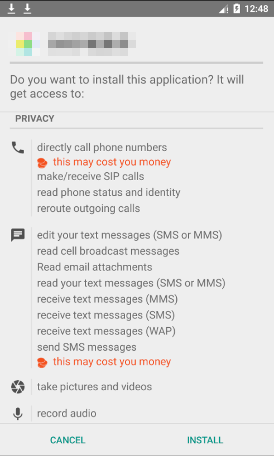
\includegraphics[width=0.3\columnwidth]{Chapter14/graph/android5.png} \\
	\end{center}
	\vspace{-10pt}
	\caption{Android 5.1 下安装应用程序} \label{fig:android5}
	\vspace{-10pt}
\end{figure}

为了解决这些问题,Android操作系统在6.0版本中引入了\textcolor{myblue}{\textbf{运行时权限}}(Runtime Permission)。这意味着用户可以在应用程序运行时对其敏感行为进行拦截。这种机制大大提高了权限管理的灵活性,一定程度上缓解了移动平台上权限滥用的局面。

谷歌公司最新开发的Android 12 当中还引入了``隐私信息中心''这一功能,以便直观地呈现应用程序索取隐私信息的情况。如图\ref{fig:android12}所示,用户可以查看最近有哪些程序访问了摄像头、麦克风以及地理位置信息。这一功能进一步加强了权限管理的约束力,对规范应用程序的隐私获取行为有一定的帮助。

\begin{figure}[H]
	\begin{center}
		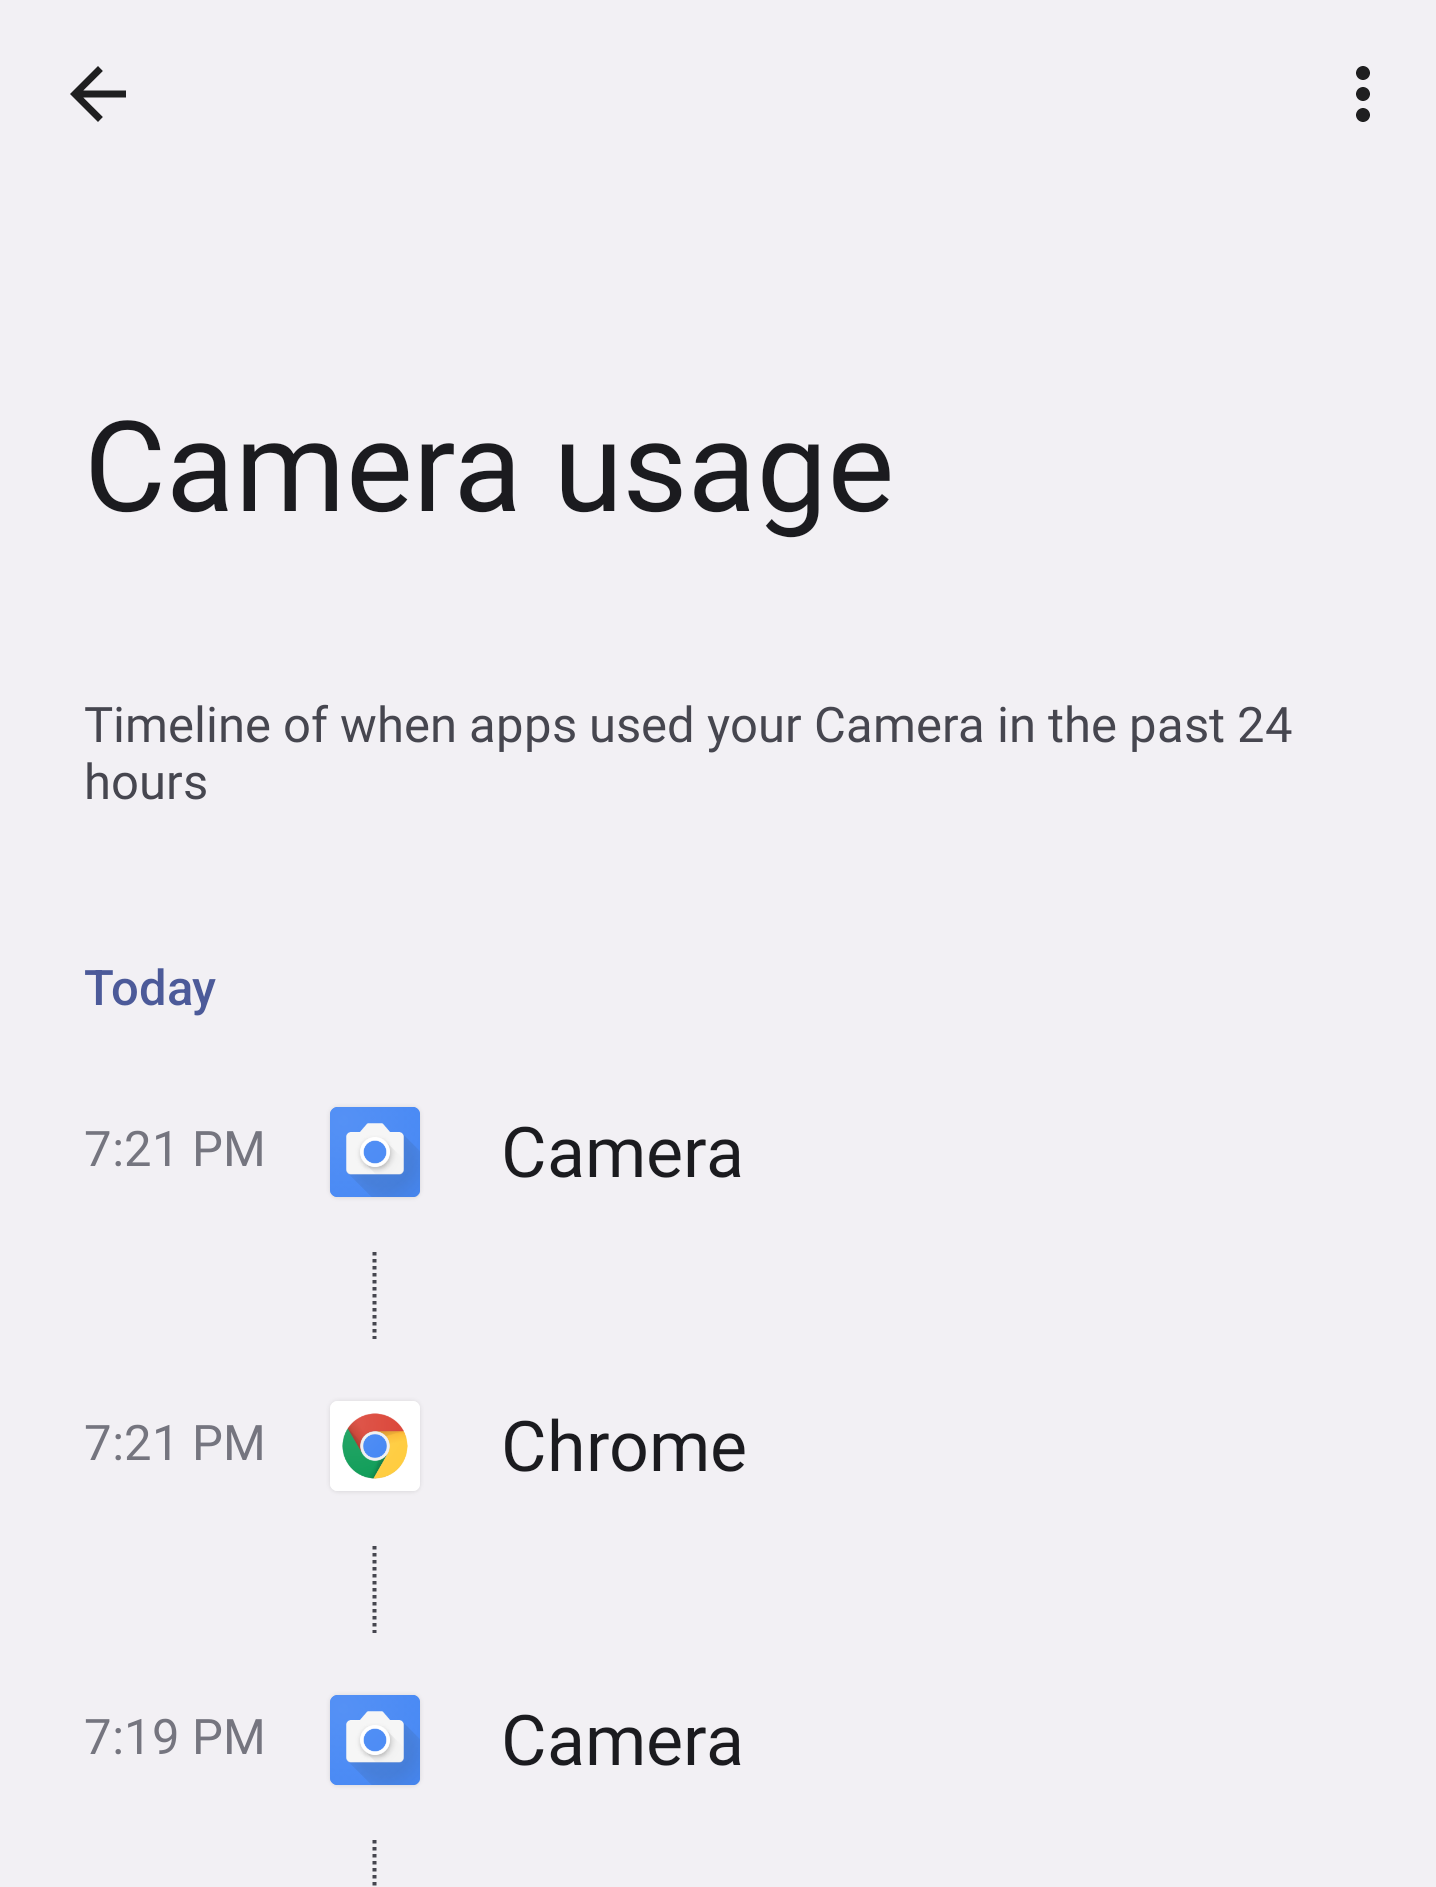
\includegraphics[width=0.3\columnwidth]{Chapter14/graph/android12.png} \\
	\end{center}
	\vspace{-10pt}
	\caption{Android 12 下的隐私信息中心} \label{fig:android12}
	\vspace{-10pt}
\end{figure}


然而,最近的一些研究工作表明,权限管理功能的作用仍是相当有限的。\cite{userbehavior}当中指出,对于不合理的权限索取,仅有不到一半的用户选择了拒绝。大量的用户认为授权操作较为繁琐,从而选择了``始终允许''。由此可以看出用户的隐私保护意识普遍不强。

更为不幸的是,即使用户有足够强的隐私防护意识,也常常无法避免隐私数据的泄漏。一方面,Android系统的权限管理机制在具体实现上仍存在一些漏洞。攻击者可能通过动态分析等手段\cite{escalation},找到并利用这些漏洞,获取敏感权限。另一方面,攻击者也可以通过相对不敏感的信息来推断用户的隐私信息。例如加速度计,陀螺仪等零权限传感器就可能被利用,来达成跟踪用户,窃听环境声音等目的\cite{sensorid,eavesdrop}。
% 当中通过对Android系统权限管理机制的动态分析,发现了一些实现上的漏洞,恶意软件开发者可能利用这些漏洞获取敏感权限。也有一些工作通过相对不敏感的数据来推断敏感的隐私信息。例如通过零权限传感器(例如加速度传感器、陀螺仪等等)来达成跟踪用户、窃听环境声音等目的。
除此之外,一些软件厂商之间还结成了收集用户隐私信息的联盟,以便互通有无。对于某些业务逻辑确需获取的隐私信息(如语音通话应用程序采集到的语音信息,地图导航应用程序采集到的地理位置信息等等),用户也无从得知软件厂商是否会用作其他用途。

可以看出,随着Android系统的不断迭代,其权限管理功能也日趋完善。但是,它仍然存在着很强的局限性。因此,我们还有必要探索其他技术上或管理上的新机制,以便更好地保护用户的隐私。

\subsection{用户与设备认证}
\label{common_security}

\subsubsection{\textcolor{myblue}{\textbf{1.用户身份认证}}}


用户身份认证是保障通讯网络系统安全的根本前提,其目的在于建立各方的信任关系。在物联网环境中,用户必须通过相应的身份验证机制才能获得系统分配的资源和授予的访问权限,进而取得与设备交互的能力。攻击者也通常将身份认证系统作为集中攻击目标,通过中间人攻击、重返攻击、口令猜测攻击等方式,非法获取数据甚至控制设备实施恶意行为。

目前用户认证方案主要存在以下问题:一是缺乏统一的标准规范,导致优质资源分散,难以树立行业标杆。二是受限于有限的计算能力和存储空间,大部分设备只支持轻量级认证方案。三是随着攻击手段的迭代更新,已有设备未必适用新的安全方案或不能及时更新,需要通过更换设备实现。四是物联网的三层架构与计算机网络七层架构不同,许多计算机网络架构下认证方案的可迁移性不足,需要更有针对性地设计适配的认证方案。五是物联网设备异构化强,不同厂商间的通信协议和操作系统通常不同,需要设计兼容性更强的认证方案。

主流用户身份认证方式可根据认证过程发生的位置大致分为两种:一是本地认证,用户可通过预设密码,使用智能卡等物理外设,以及使用指纹和虹膜等生物信息的方式,和设备中预留密钥进行比对认证;二是联网认证,即通过密码学手段对用户提供的秘钥、口令、生物特征等信息进行加密,再同预留在云服务器或边缘网关中的密钥进行匹配。

上述两种认证方式的支撑技术主要有以下几类:一是基于密码的用户身份认证,即用户提供唯一ID与密码组合同预留组合进行匹配认证。二是基于MAC地址或IP地址等公开信息进行认证,这种方式是将硬件地址或网络地址与用户身份进行绑定,安全性和灵活性都相对较弱。三是基于口令的认证,该方法可分为动态和静态两类:动态口令指用户可通过持有相同的口令生成器或经由其它渠道获取一次一密的口令来完成认证;静态口令指用户使用加密狗、智能卡等存储固定口令的方式进行认证。四是基于生物特征的认证,即利用采集设备对指纹、虹膜或声纹等用户独有的生物特征进行获取,并同特征模板库进行匹配实现认证。目前,基于深度学习的多模态用户认证方案正成为该领域热门研究方向之一。上述四种方式多用于本地认证或联网认证的接入阶段,其主要目的在于根据用户所知、所有或特征信息作为准入凭证,而下述两类技术则更专注于为这些凭证提升可信程度。五是基于区块链技术设计用户认证系统,利用分布式账本抗抵赖的特性提升系统审计能力。六是使用密码学方法提升认证凭证安全性,即利用哈希算法、对称和非对称密码算法对用户提供的认证凭证进行加解密计算,如利用椭圆曲线加密,秘密共享和秘钥分割等方式进行认证。另外,利用量子密码进行用户认证的方式也逐渐成为主要研究方向之一。

目前,现有技术虽具备一定的防护能力,但长远看来,随着传感器种类的丰富与设备数量的激增,物联网环境下的用户认证方案也将面临更艰巨的考验。从现阶段发展状况看,用户身份认证系统大致有如下发展趋势:一是更注重数据安全和隐私保护;二是利用轻量级加密算法实现轻量级认证;三是通过降低计算成本等方式提升认证效率;四是提升对大量节点与海量接入的管理能力,可以更便捷地实现节点纳新;五是提升异构方案适配能力,兼容多平台和多协议,开发友好API;六是机器学习、区块链和量子计算等新技术将进一步推进用户认证系统发展;七是增强系统鲁棒性;八是提升审计能力。

\subsubsection{\textcolor{myblue}{\textbf{2.设备身份认证}}}

用户身份认证至关重要,而互联设备的身份认证也极其重要。在物联网环境中,各设备之间存在大量点对点通信,为了避免指令混乱甚至恶意攻击,设备在执行指令之前必须确保互联设备的真实性。因此,对设备提取设备指纹并进行设备身份认证至关重要。目前,设备指纹主要分为软件指纹和硬件指纹两类。

软件指纹是指人为对设备设定的识别标识,包括:唯一标识密钥(安全令牌)、国际移动设备标识(IMEI)、MAC地址、浏览器指纹等。
其中,唯一标识密钥用于同一网络内设备之间的身份认证,设备可使用该密钥进行安全通信。
国际移动设备标识是一种和设备相关的唯一标识,相当于用户的唯一ID,在通信时通过验证IMEI码即可确认互联设备身份。
同样的,MAC地址是联网设备的一种唯一标识,用于网络配置。因为其唯一性,也常用于设备身份验证。
而浏览器指纹是通过浏览器和Cookie获取设备软硬件设置等信息来识别设备。
以上这些设备指纹都存在一定的安全风险,比如:安全令牌一旦泄露,整个网络通信将不再可信。
IMEI码和MAC地址的篡改也并不困难。
在用户隐私保护意识较强的今天,许多用户会选择关闭Cookie记录,这直接导致浏览器指纹的可靠性大幅降低。
因此,以上软件指纹普遍存在易被篡改、可靠性低等问题,设备认证整体安全性较低。

硬件指纹是指物联网设备硬件与生俱来的一种特性,这种特性存在于每台设备中,且设备之间各不相同。
这种硬件指纹来源于传感器等部件生产的不完美性,验证端可以从传感器采集的数据中提取硬件指纹。
常用的设备硬件指纹有:相机指纹、音频指纹、运动传感器指纹等。
其中,相机指纹是摄像头上的硬件指纹。摄像头最重要的感光元件由几百万个像素点组成,由于生产工艺的不完美性,每个成品的感光元件不可能完全一致,像素点之间细微的透光差异将在拍摄的每张照片中留下痕迹。这种唯一且与生俱来的痕迹称为相机指纹。通过对照片提取相机指纹,就可以判断摄像头所在设备的身份。
音频指纹由麦克风和扬声器组合生成,它们拥有相似的结构,都由磁钢和线圈组成,但每个磁钢与线圈之间的距离存在一定差异,具体体现在播放与录音的结果中。即使播放相同的音频,扬声器输出的声音并不相同。同理,即使在相同距离接收同一声音,不同麦克风收录的内容也有差异。两者组合时,扬声器播放相同音频,麦克风同时录制,就可以得到录音对应的独特频率响应曲线,并作为硬件指纹进行设备认证。
运动传感器主要包括加速度传感器和陀螺仪。同样因为生产的不完美性导致个体差异,成品件对相同运动的响应存在差异。因此,在相同震动情况下,不同传感器采集到的震动信息不同,可以作为设备硬件指纹进行身份认证。
这类硬件指纹不由人工设定,没有重复性也无法篡改与伪造,属于安全性较高的设备验证指纹。
 
 
\subsection{前沿研究}
物联网中的资源调度要经过权限管理和认证两个步骤。在这一节中,首先介绍权限管理相关的前沿工作,然后说明近年来学术界在设备和用户认证方面的研究成果。

近年来许多研究表明,仅依赖权限管理并不能完全解决物联网的安全和隐私问题。现有的权限管理机制依据传感组件权限的敏感程度经验性地将其划分为高权限(相机、麦克风、扬声器)及零权限(加速度计,陀螺仪和磁力计等)两类。仅有少量的研究是利用高权限传感组件窃取用户个人隐私的\cite{yu2016writinghacker,song2016my,yu2019indirect,schlegel2011soundcomber,guri2017speake},低权限传感器的隐私泄露问题是近年来国内外学者关注的热点之一。许多工作都是利用智能设备内置的陀螺仪或加速计来采集震动信号,识别乃至重建语音信息\cite{michalevsky2014gyrophone,zhang2015accelword,feng2017continuous,anand2018speechless,Ba2020Learning}。除零权限运动传感器外,一些研究还分别探索了其它异构传感组件用于窃取语音信息的可能性,例如高帧率摄像机\cite{davis2014visual}、激光雷达\cite{sami2020spying}、振动马达\cite{2016Listening}。除音频信息以外,还可以利用零权限传感器推断用户输入的数字及文本等敏感信息\cite{Xu2012Taplogger,Miluzzo2012Tapprints,Owusu2012Accessory,Cai2011TouchLogger}、运动行为\cite{kwapisz2011activity,shoaib2013towards}以及位置信息\cite{han2012accomplice}。

设备和用户认证是物联网是极其关键的一环,一直以来深受国内外学者关注。对于设备认证而言,由于硬件其本身物理不可克隆的特性,硬件指纹成为设备认证的一大研究热点。例如,部分工作利用扬声器和麦克风的听觉指纹来进行设备认证\cite{Das2014Do,Zhou2014Acoustic,Chen2015Wireless},同时智能设备内置相机的光响应非均匀性也被作为硬件指纹用于认证\cite{Ba2018ABC}。另外,软件指纹也有较多的研究成果,一些研究围绕轻量的多密钥认证模式展开研究\cite{Hammi2020A,Shah2018Authentication},区块链技术也被用于设备认证\cite{Li2018A}。

对于用户认证而言,近年来大多数研究利用智能设备的传感组件,通过捕捉生物行为特征,实现了连续和隐式的用户身份验证。大多数研究利用加速度计、陀螺仪和传感器来寻找用户的行为模式,从而进行用户认证,例如挥舞手势\cite{Hong2015Waving}、自由手势\cite{Meidan2017Detection}、拾起动作(即拿起手机并举起手机接听)\cite{Francois2010Machine}、手指按压屏幕\cite{Liu2017Vibwrite}。除此之外,眼睛移动的模式也被用于识别用户身份\cite{Zhang2018VR,Song2016Phone}。
\section{物联网隐私保护技术}
\label{protocol_security}
随着物联网隐私安全引起越来越多的关注,相应的隐私保护技术也在快速发展。
传统隐私保护技术主要利用密码学方法实施端到端加密以保护不安全的通信,从而保护用户隐私,如同态加密、安全多方计算等。而物联网隐私保护由于其资源限制大、网络节点数目多等特点无法直接使用传统隐私保护技术,需要发展适用于物联网的隐私保护技术。


本节将从以下几个方面介绍目前物联网隐私保护技术的发展情况:首先介绍目前物联网隐私保护面临的新情况与新挑战,然后介绍物联网隐私数据的具体分类,最后介绍现有的物联网轻量级隐私保护技术与目前物联网隐私保护领域的最新成果。


\subsection{物联网隐私保护新特点}
\label{common_security}

随着物联网的应用,物联网在方便用户的同时,也记录着与用户隐私相关的大量数据,这使得数据隐私安全问题迫在眉睫。2015年至今,国内外发生多起智能玩具、智能手表等漏洞攻击事件,超百万家庭和儿童信息、对话录音信息、行动轨迹信息等被泄露;我国某安防公司制造的物联网摄像头存在多个漏洞,黑客仅凭默认密码登录设备即可访问摄像头的实时画面。此外,据有关数据显示,10000户家庭每天大约能生成多达1.5亿个离散数据点。IDC报告显示,2020年全球物联网设备将有200亿~250亿台。庞大的物联网设备规模意味着有海量用户的不计其数的隐私数据被收集记录,隐私数据泄漏的风险系数被急剧放大。因此,在万物互联把数据的收集和分析的触角延伸到人们生活的各种场景同时,安全和个人数据的保护不善威胁着物理终端设备背后人们的真实生活和生命财产。与传统互联网相比较,物联网的安全问题更加复杂。在IoT场景下,我们面临的三大安全和隐私挑战是:终端认证,网络攻击预防和家庭个人数据保护。这三大挑战分别着眼于物联网“端、网、云”的三层网络架构~\cite{wenti2019}:
\par1.从“端”来看,不同物联网终端设备的安全防护能力参差不齐,差异较大。在物联网中,终端设备负责感知环境信息,例如感应、识别物体,获取环境湿度、温度等,由此产生了种类繁多的物联网设备,包括RFID芯片、指纹扫描器、温度湿度传感器、网络摄像头等。然而,大多终端设备应用场景简单,存储与计算能力有限,无法满足部署安全软件或者高复杂度的加解密算法的算力与存储需求。此外,物联网终端的‘移动’属性,消解了传统网络边界,使得依托于网络边界的安全产品无法正常发挥作用,如果物联网终端处在无人监控的环境中,则攻击者更容易对其实施攻击。
\par2.从“网”来看,物联网网络结构复杂且通信协议安全性差。相比互联网,物联网网络采用多种异构网络,更为复杂,存在算法破解、协议破解等风险以及中间人攻击等攻击威胁,Key、协议、核心算法、证书等暴力破解的情况时有发生。因此,物联网数据传输管道的防护安全与管道中的流量内容安全问题不容忽视。
\par3.从“云”来看,云平台层安全风险对于整个网络生态不容忽视。云平台通常通过网络汇集终端设备获取的感知数据,然后借助App与云平台进行信息交互,达到远程管理设备的目的。目前,云安全技术水平日益成熟,但更多的安全威胁往往来自内部的不当管理或外部渗透攻击技术。如果企业内部管理机制不完善、系统安全防护不配套,那企业内部管理过程逻辑漏洞就可能让平台或整个生态彻底沦陷。此外,依托于社会工程学的非传统网络攻击始终存在,这给系统的安全防护策略带来极大的挑战。\par

在这种物联网环境下,对于个人隐私数据的保护需要对数据进行科学分类,有效的数据分类方法有利于防护手段向灵活精细方向发展,促进系统整体防护能力的提升。\par
    

\subsection{物联网隐私数据分类}
\label{common_security}


\textcolor{myblue}{\textbf{隐私数据}}指个人或团体不愿意被他人获得的敏感信息。区别于普通数据,隐私数据常常由私人设备产生,如手机,平板电脑等,有时也可能由一些传感器产生,如摄像头等。物联网隐私数据数量庞大种类繁多\cite{qian2013},根据是否随时间变化可以分为\textcolor{myblue}{\textbf{动态数据}}和\textcolor{myblue}{\textbf{静态数据}}\cite{min2021};根据是否包含生物特征可以分为\textcolor{myblue}{\textbf{生物特征数据}}和\textcolor{myblue}{\textbf{非生物特征数据}}\cite{Preserving2019};根据能否确定一个人的身份可以分为\textcolor{myblue}{\textbf{个人数据}}和\textcolor{myblue}{\textbf{非个人数据}}\cite{Protecting2019}。


\subsubsection{\textcolor{myblue}{\textbf{1. 动态数据和静态数据}}}
\textcolor{myblue}{\textbf{动态数据}}(dynamic data):动态数据随着时间常常发生变化,如用户的实时位置。

\textcolor{myblue}{\textbf{静态数据}}(static data):静态数据指在一定时间段内不容易发生变化,如用户的的姓名、性别和家庭地址等。
\subsubsection{\textcolor{myblue}{\textbf{2. 生物特征数据和非生物特征数据}}}
\textcolor{myblue}{\textbf{生物特征数据}}(biometric data):生物特征数据指生物与生俱来与众不同的行为和特征,如声音特征、指纹、面部特征等,通常可以用来认证或识别用户的个人身份。生物特征数据一旦发生泄漏,在安全性方面可能变得毫无用处,因为它常常是不可更新的。

\textcolor{myblue}{\textbf{非生物特征数据}}(non-biometric data):除生物特征数据以外的数据为非生物特征数据,如说话时的内容、情绪,密码等。
\subsubsection{\textcolor{myblue}{\textbf{3. 个人数据和非个人数据}}}
\textcolor{myblue}{\textbf{个人数据}}(personal data):个人数据指可以唯一确定一个人身份的数据,如一个人的邮箱地址、手机号等。

\textcolor{myblue}{\textbf{非个人数据}}(non-personal data):不能确定一个人身份的数据。值得注意的是,当一些非个人数据组合在一起,有时也可以确定一个人的身份。如姓名和公司都不是个人数据,但组合在一起很大概率可以确定一个人。

针对这些隐私数据,目前已经提出了很多隐私保护方法,但在物联网中,资源常常是有限的,所以通常采用一些轻量级的方法。需要说明的是,现在的隐私保护方法不一定细化到针对各个类别的数据用不同的策略进行保护,但是为了开发出灵活有效的物联网轻量级保护方案,这是一个值得研究的方向。

 
 
\subsection{物联网轻量级隐私保护技术}
保护物联网隐私数据的常用解决方案是实施端到端加密以保护不安全的通信。
端到端加密可以分为非对称加密和对称加密。在非对称加密通信过程,当实体A尝试与另一实体B通信时,A利用B的公钥加密消息,而B利用其私钥进行解密。

公钥可以通过不可靠的通道传输,这大大方便了密钥的授权。
然而,基于非对称算法的加密和解密过程是计算密集型的,需要消耗大量的能源和计算资源\cite{luo}。
而资源受限是物联网的一大特点:由于物联网设备需与实际物品相结合,其体积受到较大限制,且大多数物联网设备需在无充电情况下维持长时间工作,
其用于加密计算的资源大大受限。
有研究表明非对称加密的计算消耗至少是对称密钥方案的100倍\cite{hirani}。
因此,对称加密是目前主流的物联网隐私保护技术轻量化发展方向。 


将对称加密用于物联网隐私保护面临的主要挑战是设计一种健壮的密钥交换机制。
当网络中某个节点被捕获时,与之通信节点的对称密钥也将泄露。
为了抵御节点捕获攻击,研究者提出了一种大规模物联网动态随机密钥建立机制,该机制支持传感器节点的多阶段部署,
通过动态分配密钥,在另一个部署阶段发生之前,部署阶段中已经部署的节点在密钥环中刷新自己的密钥\cite{das}。
另一种应对节点捕获攻击的方法是通过网络中所有节点协同生成全局密钥,该方法从网络末端节点开始生成密钥,向根节点传递并最终生成全局密钥,当有节点离开或加入网络时重新生成全局密钥\cite{hendaoui}。
而为了提高对称密钥生成效率,Kronecker积被用于分解对称矩阵,分解得到的因子矩阵中的参数分配至网络中各个节点作为密钥\cite{tsai}。


混沌系统也被用于轻量化物联网隐私保护技术。混沌系统对初始条件非常敏感,这意味着两个输入稍有不同的混沌系统的输出可能会显著不同,非常适合用于密钥生成。
此外,在基于混沌的密码系统中,即使恢复了其中一个密钥,攻击者恢复其他密钥的可能性也微乎其微,对节点捕获攻击有较强的抵抗能力。
研究者首先针对智能家居系统设计了基于混沌系统的对称加密机制,该机制利用混沌系统生成密钥,并通过消息认证码来进行节点设备认证并确保数据完整性\cite{song}。
近期,适用于大型物联网网络的基于混沌系统的对称加密机制被提出。

该机制首先利用混沌系统为每个物联网设备分配参数与初始值(即密钥)作为默认配置。
当设备首次连接到控制中心(如云平台)时,该参数和初始值用于设备注册认证。
之后,该控制中心为设备间通信分配另一对参数和初始值作为通信密钥,并使用特定参数和初始值迭代混沌系统,同步更新所有密钥\cite{luo}。


以上提出的轻量化物联网隐私保护方法仍面临只适用于小型网络或只适用于中心架构网络等问题,需要进一步的发展与完善。

\subsection{前沿研究}
\label{recentwork}

为了在物联网设备的有限资源下可靠实时地保护隐私数据,研究者们提出了诸多新的解决方案。一方面,为使得隐私保护更具实践性,研究者们在传统的物联网隐私保护技术基础上进行改进创新;另一方面,随着机器学习、区块链等技术的迅猛发展,这些技术被融入物联网中,为隐私数据提供更可靠的保障。

传统的物联网隐私保护技术包括数据匿名化、密码技术等。数据匿名化在用户和服务提供方之间引入了更多的匿名参与者以保护用户的轨迹和内容隐私,如k-匿名技术\cite{Zhang2017}。但使用数据匿名化技术保护隐私的代价是信息量的损失,而对隐私数据加解密却能无损地保护隐私。密码技术被广泛用于物联网和云服务器场景下的认证方案中以抵御离线密码猜测攻击,如椭圆曲线密码\cite{Kumari2018}。密码技术中,块密码及非对称密码的加解密速度慢,很难满足物联网设备对实时性的要求;而流密码由于其可在硬件上高效加解密的特性,从而在物联网设备中得到了广泛应用。一些流密码算法,如RCCM和PARCCM\cite{Liu2020},与边缘计算结合实现了高效地保护隐私。

物联网设备可以通过应用机器学习或深度学习算法保护隐私数据,这些算法将对接入点收集的信息进行处理,从而准确有效地鉴别出隐私威胁。例如,在VANET的场景下,车辆节点间的协作学习将会引发隐私问题,给予恶意节点根据观察到的信息推断敏感信息的机会。因此,分布式ML算法的协作IDS\cite{Tao2018}利用本地数据和共享知识检测恶意节点并保护隐私。和传统机器学习算法相比,深度学习在多项研究中都表现出了更优的速度和准确率。但无论是机器学习还是深度学习算法,算法自身会受到如对抗性攻击等威胁,这将为物联网隐私安全带来新的漏洞。


随着区块链在物联网中的融入,区块链的去中心化、信息不可篡改等优良特性将给予物联网隐私数据以更可靠的保护。区块链的去中心化特征可以帮助抵抗恶意参与者的操纵和伪造,而区块链的身份和访问管理系统将能更好地应对挑战并保护隐私数据\cite{Kshetri2017}。例如,在P2P数据共享车载网络场景下,由于车辆系统的资源限制,数据被转发至边缘计算机,此过程中恶意节点极易窃取隐私数据。因此,车载物联网数据共享方案\cite{Kang2018}利用联盟链的优势,只允许指定节点执行审计和验证的工作,并使用智能合约以确保用户的真实性。然而,仍存在一些问题导致区块链难以实际应用于物联网隐私保护中,如区块链对存储和计算资源要求高,速度慢,自身可能存在漏洞等等。


\section{总结}
\label{xj_ch2}
\section{习题}
%\markboth{习题}{习题}

\begin{enumerate}
	\item {习题1}
	\item {习题2}
	
\end{enumerate}

%\begin{thebibliography}{999}\label{ckwx}
%   \bibitem{ref1}
%	杨伟,何杰,万亚东,王沁.物联网通信协议的安全研究综述[J].计算机科学,2018,45(12):32-41.
%	\bibitem{ref2}
%	SALEEM S,ULLAHS,KWAK K S.A study of IEEE 802.15.4security framework for wireless body area networks[J]. Sensors,2011,11(2):1383-1395.
%	\bibitem{ref3}
%	YANG W, WANG Q, Ql Y, et al. Time Synchronization Attacks in lEEE802.15.4eNetworks[C]//International Conference on ldentification, Information and Knowledge in the Internet of Things. IEEE,2014:166-169.
%	\bibitem{ref4}
%	JO M, HAN L, TANN D, et al. A survey: energy exhausting attacks in MAC protocols in WBANs[J].Telecommunication Systems,2015,58(2):153-164.
%	\bibitem{ref5}
%	LE A, LOO J LASEBAE A, et al. The Impact of Rank Attack on Network Topology of Routing Protocol for Low-Power and Lossy Networks[J]. IEEE Sensors Journal, 2013,13(10):3685-3692.
%	\bibitem{ref6}
%	WALLGREN L, RAZA S, COIGT T. Routing Attacks and Countermeasures in the RPL-Based Internet of Things[J]. International Journal of Distributed Sensor Networks,2013,2013(2):167-174.
%    
%    \bibitem{witrack}
%    Adib F, Kabelac Z, Katabi D, et al. 3D tracking via body radio reflections[A]. Proceedings of the 11th USENIX Conference on Networked Systems Design and Implementation[C]. USA: USENIX Association, 2014: 317–329.
%    \bibitem{wihear}
%    Wang G, Zou Y, Zhou Z, et al. We can hear you with Wi-Fi![A]. Proceedings of the 20th annual international conference on Mobile computing and networking[C]. New York, NY, USA: Association for Computing Machinery, 2014: 593–604.
%    \bibitem{lightcommands}
%    Sugawara T, Cyr B, Rampazzi S, et al. Light Commands: Laser-Based Audio Injection Attacks on Voice-Controllable Systems[A]. S. Capkun, F. Roesner. 29th USENIX Security Symposium, USENIX Security 2020, August 12-14, 2020[C]. USENIX Association, 2020: 231–2648.
%    \bibitem{rolling colors}
%    Rolling Colors: Adversarial Laser Exploits against Traffic Light Recognition[A]. 2022.6
%    \bibitem{ExpPrinter}
%    MÜLLER J, MLADENOV V, SOMOROVSKY J, et al. SoK: exploiting network printers[C]//2017 IEEE Symposium on Security and Privacy. Piscataway: IEEE Press, 2017: 213-230.
%    \bibitem{PriviSep}
%    YAO Y, ZHOU W, JIA Y, et al. Identifying privilege separation vulnerabilities in IoT firmware with symbolic execution[C]//European Symposium on Research in Computer Security. Berlin: Springer, 2019: 638-657.
%    \bibitem{CrossBin}
%    REDINI N, MACHIRY A, WANG R, et al. Karonte: detecting insecure multi-binary interactions in embedded firmware[C]//2020 IEEE Symposium on Security and Privacy. Piscataway: IEEE Press, 2020:1544-1561.
%    \bibitem{muRAI}
%    ALMAKHDHUB N S, CLEMENTS A A, BAGCHI S, et al. μRAI: securing embedded systems with return address integrity[ C]//Proceedings 2020 Network and Distributed System Security Symposium. Virginia: the Internet Society, 2020: 1-18.
%    
%    \bibitem{hassan2018security}
%    Hassan S S, Bibon S D, Hossain M S, et al. Security threats in Bluetooth technology[J]. Computers \& Security, 2018, 74: 308-322.
%	\bibitem{giese2019security}
%	Giese D, Liu K, Sun M, et al. Security analysis of near-field communication (NFC) payments[J]. arXiv preprint arXiv:1904.10623, 2019.
%	\bibitem{zhou2008securing}
%	Zhou Y, Fang Y, Zhang Y. Securing wireless sensor networks: a survey[J]. IEEE Communications Surveys \& Tutorials, 2008, 10(3): 6-28. 
%	\bibitem{seo2014effective}
%	Seo S H, Won J, Sultana S, et al. Effective key management in dynamic wireless sensor networks[J]. IEEE Transactions on Information Forensics and Security, 2014, 10(2): 371-383.
%	\bibitem{agrawal2012a}
%	Agrawal S, Roman R, Das M L, et al. A novel key update protocol in mobile sensor networks[C]//International Conference on Information Systems Security. Springer, Berlin, Heidelberg, 2012: 194-207.
%	\bibitem{kim2017a}
%	Kim J, Song J S. A dual key-based activation scheme for secure LoRaWAN[J]. Wireless Communications and Mobile Computing, 2017, 2017.
%	\bibitem{lee2021deep}
%	Lee W, Baek S Y, Kim S H. Deep-Learning-Aided RF Fingerprinting for NFC Security[J]. IEEE Communications Magazine, 2021, 59(5): 96-101.
%	\bibitem{singh2018near}
%	Singh M M, Adzman K, Hassan R. Near Field Communication (NFC) technology security vulnerabilities and countermeasures[J]. International Journal of Engineering \& Technology, 2018, 7(4.31): 298-305.
%	\bibitem{supply2018bandwidth}
%	Supply H E. Bandwidth Spoofing and Intrusion Detection System for Multistage 5G Wireless Communication Network[J]. IEEE Wireless Communications, 2018: 2.
%	\bibitem{kumar2020NB-IoT}
%	Kumar V, Jha R K, Jain S. NB-IoT security: A survey[J]. Wireless Personal Communications, 2020, 113(4): 2661-2708.
%	\bibitem{rajashree2018security}
%	Rajashree S, Soman K S, Shah P G. Security with IP address assignment and spoofing for smart IOT devices[C]//2018 international conference on advances in computing, communications and informatics (ICACCI). IEEE, 2018: 1914-1918.
%	\bibitem{chen2020a}
%	Chen F, Huo Y, Zhu J, et al. A review on the study on MQTT security challenge[C]//2020 IEEE International Conference on Smart Cloud (SmartCloud). IEEE, 2020: 128-133.
%	\bibitem{dao2017achievable}
%	Dao N N, Kim Y, Jeong S, et al. Achievable multi-security levels for lightweight IoT-enabled devices in infrastructureless peer-aware communications[J]. IEEE Access, 2017, 5: 26743-26753.
%	\bibitem{nain2017a}
%	Nain A K, Bandaru J, Zubair M A, et al. A secure phase-encrypted IEEE 802.15. 4 transceiver design[J]. IEEE Transactions on Computers, 2017, 66(8): 1421-1427.
%	\bibitem{bui2017aes}
%	Bui D H, Puschini D, Bacles-Min S, et al. AES datapath optimization strategies for low-power low-energy multisecurity-level internet-of-things applications[J]. IEEE Transactions on Very Large Scale Integration (VLSI) Systems, 2017, 25(12): 3281-3290.
%	\bibitem{yang2017a}
%	Yang K, Forte D, Tehranipoor M M. Cdta: A comprehensive solution for counterfeit detection, traceability, and authentication in the iot supply chain[J]. ACM Transactions on Design Automation of Electronic Systems (TODAES), 2017, 22(3): 1-31.
%	\bibitem{choi2018system}
%	Choi S K, Yang C H, Kwak J. System hardening and security monitoring for IoT devices to mitigate IoT security vulnerabilities and threats[J]. KSII Transactions on Internet and Information Systems (TIIS), 2018, 12(2): 906-918.
%	\bibitem{shin2018two-factor}
%	Shin S, Kwon T. Two-factor authenticated key agreement supporting unlinkability in 5G-integrated wireless sensor networks[J]. IEEE Access, 2018, 6: 11229-11241.
%	\bibitem{glissa20196lowpsec}
%	Glissa G, Meddeb A. 6LowPSec: An end-to-end security protocol for 6LoWPAN[J]. Ad Hoc Networks, 2019, 82: 100-112.
%	\bibitem{qiu2016a}
%	Qiu Y, Ma M. A mutual authentication and key establishment scheme for M2M communication in 6LoWPAN networks[J]. IEEE transactions on industrial informatics, 2016, 12(6): 2074-2085.
%	\bibitem{qiu2017a}
%	Qiu T, Liu X, Han M, et al. A secure time synchronization protocol against fake timestamps for large-scale internet of things[J]. IEEE Internet of Things Journal, 2017, 4(6): 1879-1889.
%	\bibitem{tao2018accessauth}
%	Tao M, Ota K, Dong M, et al. AccessAuth: Capacity-aware security access authentication in federated-IoT-enabled V2G networks[J]. Journal of Parallel and Distributed Computing, 2018, 118: 107-117.
%	\bibitem{wu2017a}
%	Wu X, Li F. A multi-domain trust management model for supporting RFID applications of IoT[J]. PloS one, 2017, 12(7): e0181124.
%	\bibitem{hernandez2018mqtt}
%	Hernández Ramos S, Villalba M T, Lacuesta R. Mqtt security: A novel fuzzing approach[J]. Wireless Communications and Mobile Computing, 2018, 2018.
%    \bibitem{wong2020man}
%    Wong H, Luo T. Man-in-the-Middle Attacks on MQTT-based IoT Using BERT Based Adversarial Message Generation[C]//KDD 2020 AIoT Workshop. 2020.
%    
%    \bibitem{InjectRobot}
%    QUARTA D, POGLIANI M, POLINO M, et al. An experimental security analysis of an industrial robot controller[C]//2017 IEEE Symposium on Security and Privacy. Piscataway: IEEE Press, 2017: 268-286.
%    \bibitem{SecSurvey}
%    杨毅宇, 周威, 赵尚儒, 刘聪, 张宇辉, 王鹤, 王文杰, 张玉清. 物联网安全研究综述:威胁、检测与防御[J]. 通信学报, 2021, 42(8): 188-205.
%        \bibitem{wenti2019}
%	中国邮电报. 高度重视物联网网络信息安全问题. \url{http://paper.cnii.com.cn/article/rmydb_5064.html},2019
%	\bibitem{qian2013}
%	钱萍, 吴蒙. 物联网隐私保护研究与方法综述[J]. 计算机应用研究, 2013, 30(1):8.
%    \bibitem{min2021}
%	闵庆学, 李贺男. 物联网隐私数据风险及保护分析研究[J]. 通信管理与技术, 2021(4):3.
%	\bibitem{Preserving2019}
%	Preserving privacy in speaker and speech characterisation[J]. Computer Speech \& Language, 2019, 58(NOV.):441-480.
%	\bibitem{Protecting2019}
%	Protecting Privacy and Data in the Internet of Things[OL]. https://www.gsma.com/iot/iot-knowledgebase/protecting-privacy-and-data-in-the-internet-of-things, 2019-3-7.
%	\bibitem{hirani}
%	Hirani S A. Energy consumption of encryption schemes in wireless devices[D]. University of Pittsburgh, 2003.
%	\bibitem{das}
%	Das A K. A random key establishment scheme for multi-phase deployment in large-scale distributed sensor networks[J]. International journal of information security, 2012, 11(3): 189-211.
%	\bibitem{hendaoui}
%	Hendaoui F, Eltaief H, Youssef H. A collaborative key management scheme for distributed smart objects[J]. Transactions on Emerging Telecommunications Technologies, 2018, 29(6): e3198.
%	\bibitem{tsai}
%	Tsai I C, Yu C M, Yokota H, et al. Key management in Internet of Things via Kronecker product[C]//2017 IEEE 22nd Pacific Rim International Symposium on Dependable Computing (PRDC). IEEE, 2017: 118-124.
%	\bibitem{song}
%	Song T, Li R, Mei B, et al. A privacy preserving communication protocol for IoT applications in smart homes[J]. IEEE Internet of Things Journal, 2017, 4(6): 1844-1852.
%	\bibitem{luo}
%	Luo X, Yin L, Li C, et al. A lightweight privacy-preserving communication protocol for heterogeneous IoT environment[J]. IEEE Access, 2020, 8: 67192-67204.
%	\bibitem{Zhang2017}
%	Zhang S ,  Wang G ,  Alam B , et al. A Dual Privacy Preserving Scheme in Continuous Location-Based Services[C]// IEEE. IEEE, 2017:1-1.
%	\bibitem{Kumari2018} 
%	Kumari S ,  Karuppiah M ,  Das A K , et al. A secure authentication scheme based on elliptic curve cryptography for IoT and cloud servers[J]. The Journal of Supercomputing, 2017.
%	\bibitem{Liu2020}
%	Liu T ,  Wang Y ,  Li Y , et al. Privacy Protection based on Stream Cipher for Spatio-temporal Data in IoT[J]. IEEE Internet of Things Journal, 2020.
%	\bibitem{Mohammad2019}
%	Al-Rubaie M ,  Chang J M . Privacy-Preserving Machine Learning: Threats and Solutions[J]. Security \& Privacy, IEEE, 2019.
%	\bibitem{Tao2018}
%	Zhang T ,  Zhu Q . Distributed Privacy-Preserving Collaborative Intrusion Detection Systems for VANETs[J]. IEEE Transactions on Signal \& Information Processing Over Networks, 2018:1-1.
%	\bibitem{Kshetri2017}
%	Kshetri N . Blockchain's roles in strengthening cybersecurity and protecting privacy[J]. Telecommunications Policy, 2017, 41(10):1027-1038.
%	\bibitem{Kang2018}
%	Kang J ,  Yu R ,  Huang X , et al. Blockchain for Secure and Efficient Data Sharing in Vehicular Edge Computing and Networks[J]. IEEE Internet of Things Journal, 2019, 6(3):4660-4670.
%	
%	   \bibitem{opening:JuniperResearch}
%	Stefano NATIVI, Alexander KOTSEV, Petra SCUDO, Katarzyna POGORZELSKA, Ioannis VAKALIS, Alessandro DALLA BENETTA, Andrea PEREGO. “IoT 2.0 and the INTERNET of TRANSFORMATION (Web of Things and Digital Twins)”, EUR 30382 EN, Publications Office of the European Union, Luxembourg, 2020, ISBN 978-92-76-22403-7, doi:10.2760/553243, JRC120372.
%	
%	\bibitem{opening:IDCreport}
%	Reinsel D, Rydning J, Gantz J F. Worldwide global datasphere forecast, 2021–2025: The world keeps creating more data—now, what do we do with it all[J]. IDC Corporate USA, 2021.
%	
%    \bibitem{userbehavior} 
%	Cao W , Xia C , Sai T P , et al. A Large Scale Study of User Behavior, Expectations and Engagement with Android Permissions[C]. 30th USENIX Security Symposium (USENIX Security 21), 2021.
%
%	\bibitem{escalation}
%	Li R ,  Diao W , Li Z , et al. Android Custom Permissions Demystified: From Privilege Escalation to Design Shortcomings[C] IEEE S\&P. IEEE, 2021.
%	
%	\bibitem{sensorid}
%	Zhang J ,  Beresford A R ,  Sheret I . SensorID: Sensor Calibration Fingerprinting for Smartphones[C] 2019 IEEE Symposium on Security and Privacy (SP). IEEE, 2019.
%
%	\bibitem{eavesdrop}
%	Ba Z ,  Zheng T ,  Zhang X , et al. Learning-based Practical Smartphone Eavesdropping with Built-in Accelerometer[C]// Network and Distributed System Security Symposium. 2020.
%	
%    \bibitem{yu2016writinghacker}
%    Yu T, Jin H, Nahrstedt K. Writinghacker: audio based eavesdropping of handwriting via mobile devices[C]//Proceedings of the 2016 ACM International Joint Conference on Pervasive and Ubiquitous Computing. 2016: 463-473.
%    
%    \bibitem{song2016my}
%    Song C, Lin F, Ba Z, et al. My smartphone knows what you print: Exploring smartphone-based side-channel attacks against 3d printers[C]//Proceedings of the 2016 ACM SIGSAC Conference on Computer and Communications Security. 2016: 895-907.
%    
%    \bibitem{yu2019indirect}
%    Yu J, Lu L, Chen Y, et al. An indirect eavesdropping attack of keystrokes on touch screen through acoustic sensing[J]. IEEE Transactions on Mobile Computing, 2019, 20(2): 337-351.
%    
%    \bibitem{schlegel2011soundcomber}
%    Schlegel R, Zhang K, Zhou X, et al. Soundcomber: A Stealthy and Context-Aware Sound Trojan for Smartphones[C]//NDSS. 2011, 11: 17-3
%    
%    \bibitem{guri2017speake}
%    Guri M, Solewicz Y, Daidakulov A, et al. {SPEAKE (a) R}: Turn Speakers to Microphones for Fun and Profit[C]//11th USENIX Workshop on Offensive Technologies (WOOT 17). 2017.
%    
%    \bibitem{das2016tracking}
%    Das A, Borisov N, Caesar M. Tracking Mobile Web Users Through Motion Sensors: Attacks and Defenses[C]//NDSS. 2016.
%
%    \bibitem{das2015exploring}
%    Das A, Borisov N, Caesar M. Exploring ways to mitigate sensor-based smartphone fingerprinting[J]. arXiv preprint arXiv:1503.01874, 2015.
%
%    \bibitem{michalevsky2014gyrophone}
%    Michalevsky Y, Boneh D, Nakibly G. Gyrophone: Recognizing speech from gyroscope signals[C]//23rd USENIX Security Symposium (USENIX Security 14). 2014: 1053-1067.
%    
%    \bibitem{zhang2015accelword}
%    Zhang L, Pathak P H, Wu M, et al. Accelword: Energy efficient hotword detection through accelerometer[C]//Proceedings of the 13th Annual International Conference on Mobile Systems, Applications, and Services. 2015: 301-315.
%
%    \bibitem{feng2017continuous}
%    Feng H, Fawaz K, Shin K G. Continuous authentication for voice assistants[C]//Proceedings of the 23rd Annual International Conference on Mobile Computing and Networking. 2017: 343-355.
%    
%    \bibitem{anand2018speechless}
%    Anand S A, Saxena N. Speechless: Analyzing the threat to speech privacy from smartphone motion sensors[C]//2018 IEEE Symposium on Security and Privacy (SP). IEEE, 2018: 1000-1017.
%    
%    \bibitem{davis2014visual}
%    Davis A, Rubinstein M, Wadhwa N, et al. The visual microphone: Passive recovery of sound from video[J]. 2014.
%
%    \bibitem{2016Listening}
%    Roy N, Roy Choudhury R. Listening through a vibration motor[C]//Proceedings of the 14th Annual International Conference on Mobile Systems, Applications, and Services. 2016: 57-69.
%    
%    \bibitem{sami2020spying}
%    Sami S, Dai Y, Tan S R X, et al. Spying with your robot vacuum cleaner: eavesdropping via lidar sensors[C]//Proceedings of the 18th Conference on Embedded Networked Sensor Systems. 2020: 354-367.
%    
%    \bibitem{han2017pitchln}
%    Han J, Chung A J, Tague P. Pitchln: eavesdropping via intelligible speech reconstruction using non-acoustic sensor fusion[C]//Proceedings of the 16th ACM/IEEE International Conference on Information Processing in Sensor Networks. 2017: 181-192.
%    
%    \bibitem{marquardt2011sp}
%    Marquardt P, Verma A, Carter H, et al. (sp) iphone: Decoding vibrations from nearby keyboards using mobile phone accelerometers[C]//Proceedings of the 18th ACM conference on Computer and communications security. 2011: 551-562.
%    
%    \bibitem{kwapisz2011activity}
%    Kwapisz J R, Weiss G M, Moore S A. Activity recognition using cell phone accelerometers[J]. ACM SigKDD Explorations Newsletter, 2011, 12(2): 74-82.
%    
%    \bibitem{shoaib2013towards}
%    Shoaib M, Scholten H, Havinga P J M. Towards physical activity recognition using smartphone sensors[C]//2013 IEEE 10th international conference on ubiquitous intelligence and computing and 2013 IEEE 10th international conference on autonomic and trusted computing. IEEE, 2013: 80-87.
%    
%    \bibitem{han2012accomplice}
%    Han J, Owusu E, Nguyen L T, et al. Accomplice: Location inference using accelerometers on smartphones[C]//2012 Fourth International Conference on Communication Systems and Networks (COMSNETS 2012). IEEE, 2012: 1-9.
%	
%	\bibitem{Das2014Do}
%    Das A, Borisov N, Caesar M. Do you hear what I hear? Fingerprinting smart devices through embedded acoustic components[C]//Proceedings of the 2014 ACM SIGSAC Conference on Computer and Communications Security. 2014: 441-452.
%    
%    \bibitem{Zhou2014Acoustic}
%    Zhou Z, Diao W, Liu X, et al. Acoustic fingerprinting revisited: Generate stable device id stealthily with inaudible sound[C]//Proceedings of the 2014 ACM SIGSAC Conference on Computer and Communications Security. 2014: 429-440.
%    
%    \bibitem{Chen2015Wireless}
%    Chen D, Mao X, Qin Z, et al. Wireless device authentication using acoustic hardware fingerprints[C]//International Conference on Big Data Computing and Communications. Springer, Cham, 2015: 193-204.
%    
%    \bibitem{Ba2018ABC}
%    Ba Z, Piao S, Fu X, et al. ABC: Enabling smartphone authentication with built-in camera[C]//25th Annual Network and Distributed System Security Symposium, NDSS 2018. 2018.
%    
%    \bibitem{Hammi2020A}
%    Hammi B, Fayad A, Khatoun R, et al. A lightweight ECC-based authentication scheme for Internet of Things (IoT)[J]. IEEE Systems Journal, 2020, 14(3): 3440-3450.
%    
%    \bibitem{Shah2018Authentication}
%    Shah T, Venkatesan S. Authentication of IoT device and IoT server using secure vaults[C]//2018 17th IEEE International Conference On Trust, Security And Privacy In Computing And Communications/12th IEEE International Conference On Big Data Science And Engineering (TrustCom/BigDataSE). IEEE, 2018: 819-824.
%    
%    \bibitem{Li2018A}
%    Li D, Peng W, Deng W, et al. A blockchain-based authentication and security mechanism for IoT[C]//2018 27th International Conference on Computer Communication and Networks (ICCCN). IEEE, 2018: 1-6.
%    
%    \bibitem{Alizai2018Improved}
%    Alizai Z A, Tareen N F, Jadoon I. Improved IoT device authentication scheme using device capability and digital signatures[C]//2018 International Conference on Applied and Engineering Mathematics (ICAEM). IEEE, 2018: 1-5.
%    
%    \bibitem{Hong2015Waving}
%    Hong F, Wei M, You S, et al. Waving authentication: your smartphone authenticate you on motion gesture[C]//Proceedings of the 33rd Annual ACM Conference Extended Abstracts on Human Factors in Computing Systems. 2015: 263-266.
%    
%    \bibitem{Meidan2017Detection}
%    Meidan Y, Bohadana M, Shabtai A, et al. Detection of unauthorized IoT devices using machine learning techniques[J]. arXiv preprint arXiv:1709.04647, 2017.
%    
%    \bibitem{Francois2010Machine}
%    Francois J, Abdelnur H, State R, et al. Machine learning techniques for passive network inventory[J]. IEEE Transactions on Network and Service Management, 2010, 7(4): 244-257.
%    
%    \bibitem{Zhang2018VR}
%    Zhang Y, Hu W, Xu W, et al. Continuous authentication using eye movement response of implicit visual stimuli[J]. Proceedings of the ACM on Interactive, Mobile, Wearable and Ubiquitous Technologies, 2018, 1(4): 1-22.
%    
%    \bibitem{Song2016Phone}
%    Song C, Wang A, Ren K, et al. Eyeveri: A secure and usable approach for smartphone user authentication[C]//IEEE INFOCOM 2016-The 35th Annual IEEE International Conference on Computer Communications. IEEE, 2016: 1-9.
%    
%    \bibitem{Liu2017Vibwrite}
%    Liu J, Wang C, Chen Y, et al. Vibwrite: Towards finger-input authentication on ubiquitous surfaces via physical vibration[C]//Proceedings of the 2017 ACM SIGSAC Conference on Computer and Communications Security. 2017: 73-87.
%    
%    \bibitem{Xu2012Taplogger}
%    Xu Z, Bai K, Zhu S. Taplogger: Inferring user inputs on smartphone touchscreens using on-board motion sensors[C]//Proceedings of the fifth ACM conference on Security and Privacy in Wireless and Mobile Networks. 2012: 113-124.
%    
%    \bibitem{Miluzzo2012Tapprints}
%    Miluzzo E, Varshavsky A, Balakrishnan S, et al. Tapprints: your finger taps have fingerprints[C]//Proceedings of the 10th international conference on Mobile systems, applications, and services. 2012: 323-336.
%    
%    \bibitem{Owusu2012Accessory}
%    Owusu E, Han J, Das S, et al. Accessory: password inference using accelerometers on smartphones[C]//proceedings of the twelfth workshop on mobile computing systems \& applications. 2012: 1-6. 
%    
%    \bibitem{Cai2011TouchLogger}
%    Cai L, Chen H. {TouchLogger}: Inferring Keystrokes on Touch Screen from Smartphone Motion[C]//6th USENIX Workshop on Hot Topics in Security (HotSec 11). 2011.
%    
%    \bibitem{Ba2020Learning}
%    Ba Z, Zheng T, Zhang X, et al. Learning-based Practical Smartphone Eavesdropping with Built-in Accelerometer[C]//NDSS. 2020.
%
%
%
%\end{thebibliography}
